\documentclass[11pt,a4paper]{article}
\usepackage{amsmath}
\usepackage{amssymb}
\usepackage{fontspec}
\usepackage[a4paper,top=2.5cm,bottom=2.5cm,left=2.5cm,right=2.5cm]{geometry}
\usepackage{longtable}
\usepackage{array}
\usepackage{xcolor}
\usepackage{colortbl}
\usepackage{listings}
\usepackage{enumitem}
\usepackage{graphicx}
\usepackage{pdflscape}
\usepackage[hidelinks]{hyperref}

\setmainfont{Times New Roman}
\setmonofont{Consolas}[Scale=0.80]

\definecolor{hdr}{gray}{0.94}
\definecolor{codebg}{gray}{0.94}

\newcommand{\tl}{\texttt}
\newcommand{\hd}[1]{\cellcolor{hdr}#1}
\renewcommand{\arraystretch}{1.35}
\setlength{\arrayrulewidth}{0.6pt}
\setlength{\parindent}{0pt}
\setlength{\parskip}{6pt}
\setlength{\tabcolsep}{5pt}
\raggedbottom
\pagestyle{empty}
\sloppy

\lstset{
  basicstyle=\ttfamily\scriptsize,
  backgroundcolor=\color{codebg},
  numbers=left, numberstyle=\tiny, numbersep=7pt, stepnumber=1,
  breaklines=true, breakindent=0pt, breakautoindent=false,
  postbreak=\mbox{$\hookrightarrow$\space},
  frame=none, framesep=3pt, xleftmargin=16pt, framexleftmargin=16pt,
  columns=fullflexible, keepspaces=true, showstringspaces=false, tabsize=4
}

\begin{document}

\begin{center}
\textbf{CMPE3209 Computer Organization --- Proje Teslim Tutanağı}
\end{center}

\textbf{Kullanım talimatı}

Bu tutanak projenin tek resmi teslim belgesidir. Her kilometre taşında (M1, M2 ve final; tümü
pazartesi) ilgili adım doldurulur ve aynı dosya güncellenerek yeniden teslim edilir. Ayrıntılı
görev tanımları proje yönergesindedir; bu tutanak yalnızca ne istendiğini ve nereye yazılacağını
gösterir.

\begin{itemize}[leftmargin=2em,itemsep=1pt,topsep=2pt]
\item Tüm sayılar birimiyle yazılır (byte, cycle, ns, GHz). Hex değerler \tl{0x} önekiyle yazılır.
\item \textbf{Varsayım} olan her değer ``(varsayım)'' etiketiyle işaretlenir.
\item Tablolara sığmayan çıktılar (assembly listesi, objdump, CSV izi, ekran görüntüleri) Git
deposuna konur. Tutanakta dosya adıyla atıf yapılır.
\item Boş bırakılan zorunlu alan, o adımın puanını sıfırlar.
\end{itemize}

\textbf{Öğrenci bilgileri}

\begin{longtable}{|p{10.2cm}|p{5.3cm}|}
\hline
\hd{Alan} & \hd{Değer}\\
\hline
Ad Soyad & Mehmet Batuhan Özer\\
\hline
Öğrenci numarası (SID) & 5001230025\\
\hline
E-posta & \tl{batuhanozer1042@gmail.com}\\
\hline
Seçilen görev (G1--G5) & G5 --- Run-length sıkıştırma\\
\hline
Seçilen ISA ve sürümü (ör.\ RV32IM) & x86-64 (Microsoft x64 ABI, PE/COFF)\\
\hline
Derleyici ve sürümü & clang-cl, LLVM 21.1.8 (MSVC 14.44.35207)\\
\hline
Simülatör / araçlar & Visual Studio 2022 (debugger), \tl{llvm-objdump} 21.1.8; CMake 3.31.6 + Ninja 1.12.1\\
\hline
Git deposu adresi & \url{https://github.com/MBatuhanOzer/Computer_Organization_Project}\\
\hline
\end{longtable}

\textbf{Adım 0 --- Kişiye özel parametreler}

Bu adım M1 ile birlikte teslim edilir. Hatalı bir parametre, ona dayanan tüm adımları geçersiz
kılar; öğretim üyesi bu tabloyu M1'de kontrol eder.

\begin{longtable}{|p{2.0cm}|p{4.5cm}|p{4.9cm}|p{3.1cm}|}
\hline
\hd{Sembol} & \hd{Tanım} & \hd{Hesap (adımlarıyla)} & \hd{Sonuç}\\
\hline
\endhead
d & SID'in son hanesi & 500123002\textbf{5} & \textbf{5}\\
\hline
D2 & SID'in son iki hanesi & 50012300\textbf{25} & \textbf{25}\\
\hline
S & SID'in hanelerinin toplamı & 5+0+0+1+2+3+0+0+2+5 & \textbf{18}\\
\hline
N & 24 + (D2 mod 25) & 24 + (25 mod 25) = 24 + 0 & \textbf{24 eleman}\\
\hline
Cache & d'ye göre: boyut / line / mapping / line sayısı / set sayısı & d = 5 satırı & \textbf{256 byte / 16 byte / 4-way set-assoc.\ / 16 line / 4 set}\\
\hline
Write policy & d çift $\rightarrow$ write-back, d tek $\rightarrow$ write-through & d = 5 (tek) & \textbf{write-through}\\
\hline
k & (S mod 7) + 3 & (18 mod 7) + 3 = 4 + 3 & \textbf{7}\\
\hline
Interrupt türü & S çift $\rightarrow$ Timer, S tek $\rightarrow$ I/O & S = 18 (çift) & \textbf{Timer}\\
\hline
f & 1.0 + 0.1 × d GHz (varsayım) & 1.0 + 0.1 × 5 & \textbf{1,5 GHz} (varsayım)\\
\hline
T1 / T2 & T1 = 1 cycle; T2 = 20 + 5 × (d mod 4) cycle (varsayım) & T2 = 20 + 5 × 1 & \textbf{1 cycle / 25 cycle} (varsayım)\\
\hline
Nc & 2 + (S mod 7) (varsayım) & 2 + 4 & \textbf{6 çekirdek} (varsayım)\\
\hline
Görev parametresi & Seçilen göreve göre (T, P, K, yön veya R) & G5: R = 2 + (SID mod 3); 5001230025 mod 3 = 0 & \textbf{R = 2}, B = 0\\
\hline
\end{longtable}

Türetilmiş: $\tau = 1/f = 1/(1{,}5\ \text{GHz}) = \mathbf{0{,}667}$ ns (varsayım).
Tutarlılık: 256 byte / 16 byte = 16 line; 16 line / 4 yol = 4 set.

\textbf{Adres alanları} (ISA'nın adres genişliği s + w bit; 64-bit ISA'da düşük 32 bit kullanılır):

\begin{longtable}{|p{6.0cm}|p{2.8cm}|p{6.2cm}|}
\hline
\hd{Alan} & \hd{Bit sayısı} & \hd{Hesap}\\
\hline
Word (w) & \textbf{4 bit} & line boyu 16 byte $= 2^4$; adres[3:0]\\
\hline
Line (r) veya set (d) & \textbf{2 bit} & set sayısı $4 = 2^2$; adres[5:4]\\
\hline
Tag ($s - r$ veya $s - d$) & \textbf{26 bit} & $s + w = 32 \Rightarrow s = 28$; $28 - 2$; adres[31:6]\\
\hline
Toplam & \textbf{32 bit} & $26 + 2 + 4$\\
\hline
\end{longtable}

\textbf{Adım 1 --- Görev seçimi ve C programı (M1: 2 Kasım, Pazartesi)}

\textbf{1.1 Görev seçimi} (yalnızca birini işaretleyin):

\begin{itemize}[leftmargin=2em,itemsep=1pt,topsep=2pt]
\item $\square$ G1 Biyomedikal sinyal alarmı
\item $\square$ G2 Sınav notu dağılımı
\item $\square$ G3 Mesaj şifreleme ve bütünlük
\item $\square$ G4 Sıralama ve medyan
\item $\boxtimes$ \textbf{G5 Run-length sıkıştırma}
\end{itemize}

\textbf{1.2 Çözüm tasarımı} (3--5 cümle: hangi algoritma, hangi fonksiyonlar, hangi veri yerleşimi
ve neden):

Program üç global dizi üzerinde çalışır: \tl{v[24]} LCG ile üretilen $\{0,1\}$ sembollerini,
\tl{enc[24]} kodlanmış (değer, tekrar) çiftlerini, \tl{dec[24]} ise geri açılmış diziyi tutar.
\tl{rle\_encode(n)} \tl{v} dizisini tek geçişte tarar; dış döngü her koşu için bir kez döner, iç
döngü aynı sembolün tekrar sayısını sayar ve her koşu \tl{(v[i] << 8) | run} biçiminde tek bir
32-bit word'e paketlenerek \tl{enc} dizisine yazılır, böylece shift, OR ve dizi store'u aynı
satırda görünür hale gelir. \tl{rle\_decode(len)} bu paketleri \tl{>> 8} ve \tl{\& 0xFF} ile
ayrıştırıp \tl{dec} dizisine açar; her iki fonksiyon da parametre alıp değer döndürür. Doğrulama
iki aşamalıdır: önce eleman sayısı (\tl{out == N}), sonra üçüncü geçişte eleman değerleri
karşılaştırılır. Veri yerleşimi bilinçli olarak üç ayrı global dizi şeklinde seçilmiştir: üç dizi
15 cache line'a karşılık gelir, 256 byte'lık cache ise 16 line tutar; bu, 4-way set'lerden tam
birinin taşmasını sağlayarak Aşama 4'te hem spatial locality'nin hem de conflict miss'in aynı iz
üzerinde gözlenmesine imkân verir.

\textbf{1.3 C kaynak kodu.} Satır numaralı kod aşağıdaki bloğa yapıştırılır (25--60 satır):

\lstinputlisting[language=C]{main.c}

Tek dosya, C99, 54 satır kod (toplam 70 satır; 9 boş ve 6 yalnızca yorum içeren satır hariç).
\tl{clang -std=c99 -pedantic-errors -Wall -Wextra} ile uyarısız derlenir. Uzun yorum satırları
listede $\hookrightarrow$ ile sarılmıştır.

\textbf{1.4 Zorunlu yapı eşlemesi.} Her madde için satır numarası ve tek cümlelik açıklama:

\begin{longtable}{|p{0.9cm}|p{4.3cm}|p{2.2cm}|p{7.3cm}|}
\hline
\hd{\#} & \hd{Zorunlu yapı} & \hd{Satır no} & \hd{Açıklama}\\
\hline
\endhead
Y1 & N elemanlı global int dizisi, en az iki geçiş & \textbf{15}; 56, 28, 64 & \tl{s32 v[N];} --- \tl{v} üzerinde üç geçiş: s.~56 yazma, s.~28 okuma/kodlama, s.~64 doğrulama\\
\hline
Y2 & Koşullu dallanma & \textbf{30}; 65 & s.~30 \tl{v[i+run] == v[i]} koşu uzunluğunu belirler; s.~65 \tl{if (dec[i] != v[i])}\\
\hline
Y3 & Parametreli, değer döndüren fonksiyon çağrısı & \textbf{24}, 39 (tanım); \textbf{60}, 61 (çağrı) & \tl{s32 rle\_encode(s32 n)} ve \tl{s32 rle\_decode(s32 len)}; ikisi de parametre alır, değer döndürür ve dönen değer çağrı yerinde bir değişkene atanır\\
\hline
Y4 & Toplama/çıkarma, çarpma veya shift, bit işlemi & \textbf{31}, 33, 43, 44, 62 & s.~31 \tl{<< 8} ve \tl{|}; s.~33 \tl{i += run}; s.~43 \tl{>> 8}; s.~44 \tl{\& 0xFF}; s.~62 \tl{100 * enc\_len}\\
\hline
Y5 & Dizi elemanına store & \textbf{58}, 31, 46 & \tl{v[i] = ...} (s.~58), \tl{enc[k] = ...} (s.~31), \tl{dec[o++] = ...} (s.~46)\\
\hline
Y6 & \tl{const int SID} ve hesapta kullanımı & \textbf{13} (tanım), \textbf{55} (kullanım) & \tl{const int SID = 1230025;} (numara $2^{31}-1$'i aştığı için son 9 hane); LCG'nin $x_0$ tohumudur, dolayısıyla tüm \tl{v} dizisini ve üç Y7 çıktısını belirler\\
\hline
Y7 & Sonucun tutulduğu global değişken(ler) & \textbf{19, 20, 21} & \tl{enc\_len}, \tl{ratio\_x100}, \tl{decode\_ok}\\
\hline
\end{longtable}

\textbf{1.5 Program çıktıları.} Simülatörde çalıştırıldıktan sonra bellekten okunan değerler:

\begin{longtable}{|p{3.0cm}|p{2.8cm}|p{5.6cm}|p{3.3cm}|}
\hline
\hd{Global değişken} & \hd{Adres (hex)} & \hd{Değer} & \hd{Ekran görüntüsü dosyası}\\
\hline
\endhead
\tl{enc\_len} & \tl{0x140075C60} & \textbf{11} \quad(\tl{0x0000000B}) & \tl{ss\_globals.png}\\
\hline
\tl{ratio\_x100} & \tl{0x140075C64} & \textbf{45} \quad(\tl{0x0000002D}) & \tl{ss\_globals.png}\\
\hline
\tl{decode\_ok} & \tl{0x140075C68} & \textbf{1} \quad(\tl{0x00000001}) & \tl{ss\_globals.png}\\
\hline
\tl{v[24]} & \tl{0x140075C70} & \tl{0001 0001 0000 0111 0010 1110} & \tl{ss\_globals.png}\\
\hline
\tl{enc[0..10]} & \tl{0x140075CD0} & \tl{0x0003 0x0101 0x0003 0x0101 0x0005 0x0103 0x0002 0x0101 0x0001 0x0103 0x0001} & \tl{ss\_globals.png}\\
\hline
\tl{dec[24]} & \tl{0x140075D30} & \tl{v} ile birebir aynı & \tl{ss\_globals.png}\\
\hline
\end{longtable}

Değerler Visual Studio 2022 Watch penceresinden okunmuştur; pencere onlu taban kullanır
(\tl{257} $=$ \tl{0x0101}, \tl{259} $=$ \tl{0x0103}) ve \tl{enc}'in tanımlı 24 elemanının
tamamını gösterir, yalnızca ilk \tl{enc\_len} $= 11$ tanesi anlamlıdır.
\tl{ratio\_x100} $= \lfloor 100 \times 11 / 24 \rfloor = 45$; yönergedeki $R = 2$ için
``yaklaşık 50'' beklentisine göre fark, $N = 24$'ün küçüklüğünden kaynaklanan örneklem
dalgalanmasıdır (beklenen koşu sayısı 12, ölçülen 11).

\textbf{1.6 İzlenecek kernel} (12--20 dinamik instruction; en az bir load, store, ALU, koşullu
branch ve call/return içermeli):

\begin{longtable}{|p{6.0cm}|p{9.5cm}|}
\hline
\hd{Alan} & \hd{Değer}\\
\hline
C satır aralığı & s.~49 (\tl{return o;}) ve s.~61--64\\
\hline
Başlangıç ve bitiş adresi (hex) & \tl{0x140001168} -- \tl{0x140001232} (toplam 68 byte)\\
\hline
Dinamik instruction sayısı & \textbf{17}\\
\hline
Hangi döngü iterasyonu (ör.\ i = 3) & \tl{rle\_decode}'dan tek dönüş; ardından doğrulama döngüsünün ilk testi ($i = 0$)\\
\hline
\end{longtable}

İçerik kontrolü: load (\#1, 5, 10, 16), store (\#4, 9, 14), ALU (\#5 \tl{imul}, \#8 \tl{idiv},
\#12 \tl{and}), koşullu branch (\#17 \tl{jge}), fonksiyon dönüşü (\#3 \tl{ret}).
$k = 7$ interrupt'ı 7.~instruction olan \tl{cdq}'ya (\tl{0x140001208}) denk gelir; kaydedilecek
PC $=$ \tl{0x140001209}. Kernel'in tam instruction listesi ek belgededir
(\tl{M1\_Adim0\_Adim1.pdf}, Bölüm 2.6).

\textbf{Öğretim üyesi (M1):} $\square$ Onaylandı \quad $\square$ Düzeltme istendi \quad
$\square$ Reddedildi --- Tarih: \rule{2.2cm}{0.4pt} \quad Not: \rule{2.2cm}{0.4pt}

\textbf{Adım 2 --- Assembly ve machine code (M2: 9 Kasım, Pazartesi)}

\textbf{2a. C $\rightarrow$ assembly eşlemesi} (-O0; listenin tamamı depoda asm\_O0.s):

Derleme: \tl{cmake -{}-preset od} (\tl{/Zi /Od /Ob0}). Her derleme \tl{listings/} altına
derleyicinin C satır işaretli assembly'sini (\tl{asm\_O0.s}) ve linklenmiş exe'deki kendi
fonksiyonlarımızın disassembly'sini (\tl{objdump\_O0.txt}) yazar. İkisi instruction instruction
eşlenerek her C satırının gerçek adres aralığı bulunmuştur; 146 instruction'ın tamamı
\tl{listings/c2asm\_O0.txt} dosyasındadır.

{\small
\begin{longtable}{|p{1.0cm}|p{3.4cm}|p{6.6cm}|p{3.4cm}|}
\hline
\hd{C satır no} & \hd{C ifadesi} & \hd{Assembly satırları} & \hd{Adres aralığı (hex)}\\
\hline
\endhead
55 & \tl{u32 x = (u32)SID;} & \tl{mov dword ptr [rsp+0x30], 0x12c4c9} & \tl{0x14000118C}--\tl{0x140001193}\\
\hline
57 & \tl{x = 1664525u * x + 1013904223u;} & \tl{imul eax, dword ptr [rsp+0x30], 0x19660d}; \tl{add eax, 0x3c6ef35f}; \tl{mov dword ptr [rsp+0x30], eax} & \tl{0x1400011A3}--\tl{0x1400011B3}\\
\hline
28 & \tl{while (i < n) \{} & test: \tl{mov eax, [rsp+0x10]}; \tl{cmp eax, [rsp+0x14]}; \tl{jge 0x1400010C5} \newline geri dönüş: \tl{jmp 0x140001018} & \tl{0x140001018}--\tl{0x140001025} \newline ve \tl{0x1400010C0}--\tl{0x1400010C4}\\
\hline
31 & \tl{enc[k] = (v[i] << 8) | run;} & \tl{movsxd rcx, [rsp+0x10]}; \tl{lea rax, [rip+..]} (\tl{v}); \tl{mov edx, [rax+4*rcx]}; \tl{shl edx, 0x8}; \tl{or edx, [rsp+0x8]}; \tl{movsxd rcx, [rsp+0xc]}; \tl{lea rax, [rip+..]} (\tl{enc}); \tl{mov [rax+4*rcx], edx} & \tl{0x140001084}--\tl{0x1400010A8}\\
\hline
60 & \tl{enc\_len = rle\_encode(N);} & \tl{mov ecx, 0x18}; \tl{call 0x140001000}; \tl{mov [rip+..], eax} (\tl{enc\_len}) & \tl{0x1400011DD}--\tl{0x1400011EC}\\
\hline
62 & \tl{ratio\_x100 = (100 * enc\_len) / N;} & \tl{imul eax, [rip+..], 0x64}; \tl{mov ecx, 0x18}; \tl{cdq}; \tl{idiv ecx}; \tl{mov [rip+..], eax} & \tl{0x1400011FC}--\tl{0x140001210}\\
\hline
\end{longtable}
}

Satır 28 iki ayrı adres aralığına düşer: döngü testi döngünün başında, geri dönüş \tl{jmp}'i
sonundadır; tek bir C satırı bitişik olmayan makine koduna karşılık gelebilir. Satır 30'daki
\tl{\&\&} koşulu -O0'da 23 instruction'a açılır: önce sınır testi (\tl{jge}), ardından
\tl{cmp} + \tl{sete} ile sonuç bir byte'lık stack değişkenine yazılıp tekrar okunur.

{\small
\begin{longtable}{|p{1.8cm}|p{3.0cm}|p{2.6cm}|p{7.0cm}|}
\hline
\hd{Bölüm} & \hd{Başlangıç adresi (hex)} & \hd{Boyut (byte)} & \hd{İçerik}\\
\hline
\tl{.text} & \tl{0x140001000} & 395\,750 (\tl{0x609E6}) & Kendi kodumuz \tl{0x140001000}--\tl{0x140001272} (627 byte: \tl{rle\_encode}, \tl{rle\_decode}, \tl{main}); geri kalanı statik CRT\\
\hline
\tl{.rdata} & \tl{0x140062000} & 75\,452 (\tl{0x126BC}) & \tl{SID} (\tl{0x140062000}) ve CRT'nin salt-okunur verisi\\
\hline
\tl{.data / .bss} & \tl{0x140075000} & 3\,584 (\tl{0xE00}) & \tl{enc\_len} \tl{0x140075C60}, \tl{ratio\_x100}, \tl{decode\_ok}, \tl{v} \tl{0x140075C70}, \tl{enc} \tl{0x140075CD0}, \tl{dec} \tl{0x140075D30}. Sıfırla ilklenen globaller; PE'de ayrı \tl{.bss} bölümü yoktur, linker bunları \tl{.data}'ya katar.\\
\hline
\end{longtable}
}

\textbf{Von Neumann ilkesi bu adreslerde nasıl görünüyor?} Komutlar (\tl{.text},
\tl{0x140001000}) ve veriler (\tl{.rdata} \tl{0x140062000}, \tl{.data} \tl{0x140075000}) aynı tek
ve doğrusal adres uzayındadır. Bu RIP-relative adreslemede doğrudan görülür: \tl{0x1400011C6}'daki
\tl{lea rax, [rip+0x74AA3]}, \tl{v}'nin adresini bir sonraki komutun adresine sabit bir uzaklık
ekleyerek bulur (\tl{0x1400011CD} + \tl{0x74AA3} $=$ \tl{0x140075C70}); bu hesap ancak komut ve
veri aynı adres uzayında durduğunda anlamlıdır.

Program \tl{SID}'i \tl{.rdata}'dan okumaz: \tl{const int} olduğu için derleyici değeri satır
55'teki komutun içine immediate olarak gömer (\tl{c9 c4 12 00}). \tl{.rdata}'daki kopya yalnızca
\tl{SID}'in dış bağlantılı (external linkage) bir sembol olması nedeniyle üretilir.

\textbf{2b. -O0 ve -O1 karşılaştırması (kernel için):}

Kernel C satırlarıyla tanımlıdır (s.~49 \tl{return o;} ve s.~61--64); \tl{/O1} sütunu aynı C
satırlarına ait instruction'ları sayar (\tl{listings/c2asm\_O1.txt}). Load ve store sayıları
bütün bellek okuma/yazmalarını içerir; \tl{ret} ve \tl{pop} stack'ten okudukları için load sayılır.

{\small
\begin{longtable}{|p{3.4cm}|p{1.0cm}|p{1.0cm}|p{9.0cm}|}
\hline
\hd{Ölçü} & \hd{-O0} & \hd{-O1} & \hd{Farkın nedeni}\\
\hline
\endhead
Kernel'deki instruction sayısı & 17 & 18 & Register allocation spill/reload'ları kaldırdı (\tl{out} ve \tl{i} artık register'da; s.~61: 1$\to$0) ve döngü döndürüldüğü için ilk test silindi (\tl{N} $=$ 24 $>$ 0 derleme anında bilinir; s.~64: 3$\to$0). Buna karşılık \tl{/ 24} bölmesi \tl{cdq}+\tl{idiv} yerine sabitle çarpma dizisine dönüştü (\tl{imul} ile \tl{0x2AAAAAAB}, \tl{sar 34}; s.~62: 5$\to$8) ve \tl{rle\_decode} dönüşte üç callee-saved register'ı geri yükledi (s.~49: 3$\to$4). Net etki: daha az bellek erişimi, biraz daha fazla ama daha ucuz instruction.\\
\hline
Load sayısı & 5 & 5 & -O0: 3 spill okuma (\tl{o}, \tl{out}, \tl{i}) $+$ \tl{enc\_len} $+$ \tl{ret}. -O1: spill okuma 0; yerine 3 \tl{pop} (callee-saved \tl{rbx}, \tl{rdi}, \tl{rsi}) $+$ \tl{enc\_len} $+$ \tl{ret}. Sayı aynı, içerik farklı: değişken trafiği tamamen kalktı.\\
\hline
Store sayısı & 4 & 2 & -O0'da \tl{out} ve \tl{i} stack'e yazılır (2 spill store); -O1'de register'da kalırlar. Kalan 2 store \tl{ratio\_x100} ve \tl{decode\_ok}'tur ve kaldırılamaz: sonuç global değişkende tutulmalıdır (Y7).\\
\hline
Kullanılan register sayısı & 4 & 7 & -O0 her değişkeni stack'te tuttuğu için yalnızca \tl{rax}, \tl{rcx}, \tl{rdx}, \tl{rsp} kullanır. -O1 değişkenleri register'larda yaşatır: \tl{rax}, \tl{rcx}, \tl{rdx}, \tl{rsp} $+$ \tl{rbx}, \tl{rdi}, \tl{rsi}. Bu üçü callee-saved olduğu için kullanılmaları onları kaydetme/geri yükleme maliyetini (\tl{push}/\tl{pop}) beraberinde getirir.\\
\hline
\end{longtable}
}

Bellek referansı toplamı (load $+$ store): -O0'da 9, -O1'de 7. Stack üzerindeki değişken
trafiği 5'ten 0'a iner; azalmanın tamamı register allocation'dan gelir.

\textbf{2c. Elle machine code} (en az 10 instruction; x86-64 için 8). Kullanılan tüm formatlar
kapsanmalı.

Değişken uzunluklu x86-64'te ``format'', bir instruction'ın hangi alanları taşıdığıdır (prefix,
REX, opcode, ModR/M, SIB, displacement, immediate). Format sütunu Intel SDM Cilt 2'nin
``Op/En'' sınıflandırmasını kullanır. Seçilen 10 instruction programda kullanılan her alan türünü
en az bir kez içerir: REX.W (\#2), tek byte'lık opcode (çoğu), iki byte'lık \tl{0F} opcode (\#9),
ModR/M.reg içinde opcode uzantısı (\#2, \#4), opcode içinde register (\#8), ModR/M mod $=$ 00
RIP-relative (\#7), mod $=$ 01 (\#1, \#4, \#6), mod $=$ 11 (\#2, \#9), SIB (\#1, \#4, \#6), disp8
(\#1, \#4, \#6), disp32 (\#7), imm8 (\#2, \#7), imm32 (\#4, \#8), rel8 (\#10), rel32 (\#5) ve
operandsız (\#3). Instruction'ların 8'i kernel'den alınmıştır (\#4 ve \#5 hariç); doğrulama
\tl{listings/objdump\_O0.txt} ile yapılır.

{\scriptsize
\setlength{\tabcolsep}{3pt}
\begin{longtable}{|p{0.35cm}|p{1.85cm}|p{3.3cm}|p{1.9cm}|p{2.5cm}|p{1.7cm}|p{1.5cm}|p{1.0cm}|}
\hline
\hd{\#} & \hd{Adres (hex)} & \hd{Assembly} & \hd{Format} & \hd{Alanlar (ad = binary)} & \hd{Machine code (hex)} & \hd{Bellekteki byte sırası} & \hd{objdump ile aynı mı?}\\
\hline
\endhead
1 & \tl{0x140001168} & \tl{mov eax, dword ptr [rsp+0x10]} & RM: \tl{8B /r} & \tl{op=10001011} \newline \tl{mod=01 reg=000 rm=100} \newline \tl{ss=00 idx=100 base=100} \newline \tl{disp8=00010000} & \tl{8B 44 24 10} & \tl{8B, 44, 24, 10} & \checkmark \\
\hline
2 & \tl{0x14000116C} & \tl{add rsp, 0x18} & MI: \tl{REX.W 83 /0 ib} & \tl{REX=0100 W=1 R=0 X=0 B=0} \newline \tl{op=10000011} \newline \tl{mod=11 reg=000(/0) rm=100} \newline \tl{imm8=00011000} & \tl{48 83 C4 18} & \tl{48, 83, C4, 18} & \checkmark \\
\hline
3 & \tl{0x140001170} & \tl{ret} & ZO: \tl{C3} & \tl{op=11000011} & \tl{C3} & \tl{C3} & \checkmark \\
\hline
4 & \tl{0x14000118C} & \tl{mov dword ptr [rsp+0x30], 0x12c4c9} & MI: \tl{C7 /0 id} & \tl{op=11000111} \newline \tl{mod=01 reg=000(/0) rm=100} \newline \tl{ss=00 idx=100 base=100} \newline \tl{disp8=00110000} \newline \tl{imm32=0x0012C4C9} & \tl{C7 44 24 30 C9 C4 12 00} & \tl{C7, 44, 24, 30, C9, C4, 12, 00 (imm32 LE)} & \checkmark \\
\hline
5 & \tl{0x1400011F3} & \tl{call 0x1400010D0} (\tl{rle\_decode}) & D: \tl{E8 cd} & \tl{op=11101000} \newline \tl{rel32=0xFFFFFED8 (-296)} & \tl{E8 D8 FE FF FF} & \tl{E8, D8, FE, FF, FF (rel32 LE)} & \checkmark \\
\hline
6 & \tl{0x1400011F8} & \tl{mov dword ptr [rsp+0x28], eax} & MR: \tl{89 /r} & \tl{op=10001001} \newline \tl{mod=01 reg=000 rm=100} \newline \tl{ss=00 idx=100 base=100} \newline \tl{disp8=00101000} & \tl{89 44 24 28} & \tl{89, 44, 24, 28} & \checkmark \\
\hline
7 & \tl{0x1400011FC} & \tl{imul eax, dword ptr [rip+0x74a5d], 0x64} & RMI: \tl{6B /r ib} & \tl{op=01101011} \newline \tl{mod=00 reg=000 rm=101(RIP)} \newline \tl{disp32=0x00074A5D} \newline \tl{imm8=01100100} & \tl{6B 05 5D 4A 07 00 64} & \tl{6B, 05, 5D, 4A, 07, 00, 64 (disp32 LE)} & \checkmark \\
\hline
8 & \tl{0x140001203} & \tl{mov ecx, 0x18} & OI: \tl{B8+rd id} & \tl{op=10111 reg=001(ecx)} \newline \tl{imm32=0x00000018} & \tl{B9 18 00 00 00} & \tl{B9, 18, 00, 00, 00 (imm32 LE)} & \checkmark \\
\hline
9 & \tl{0x140001216} & \tl{sete al} & M: \tl{0F 94} & \tl{esc=00001111} \newline \tl{op=10010100} \newline \tl{mod=11 reg=000 rm=000(al)} & \tl{0F 94 C0} & \tl{0F, 94, C0} & \checkmark \\
\hline
10 & \tl{0x140001231} & \tl{jge 0x14000126C} & D: \tl{7D cb} & \tl{op=01111101} \newline \tl{rel8=00111001 (+57)} & \tl{7D 39} & \tl{7D, 39} & \checkmark \\
\hline
\end{longtable}
}

\textbf{Doğrulama.} Tablodaki 10 instruction'ın makine kodu, linklenmiş \tl{build-od/rle.exe}
üzerinde Visual Studio 2022 Disassembly penceresinde (\emph{Show Code Bytes} açık) birebir
doğrulanmıştır; ekran görüntüsü depoda \tl{ss\_m2\_disasm.png} dosyasındadır. Pencere C
satırlarını da gösterdiği için 2a'daki eşlemeyi de doğrular; stack değişkenleri PDB'den gelen
adlarıyla görünür (ör.\ \tl{[x]} $=$ \tl{[rsp+0x30]}, \tl{[out]} $=$ \tl{[rsp+0x28]}).

Zorunlu instruction'ların tablodaki sıra numarası:

\begin{itemize}[leftmargin=2em,itemsep=1pt,topsep=2pt]
\item $\boxtimes$ SID'i yükleyen instruction(lar): \# 4
\item $\boxtimes$ Koşullu branch: \# 10
\item $\boxtimes$ Load: \# 1
\item $\boxtimes$ Store: \# 6
\item $\boxtimes$ Fonksiyon çağrısı: \# 5
\end{itemize}

\textbf{SID'in yüklenmesi.} Sabitin neden tek instruction'a sığmadığı, nasıl bölündüğü ve
gerekiyorsa +1 düzeltmenin sign extension ile açıklaması:

x86-64'te sabit tek instruction'a \textbf{sığar}, bölünmez ve düzeltme gerekmez. \#4
(\tl{C7 /0 id}) 32 bitlik bir immediate alanı taşır; \tl{SID} $=$ 1\,230\,025 $=$
\tl{0x0012C4C9}, instruction'ın son dört byte'ına little-endian olarak yazılır:
\tl{C9 C4 12 00}. Bu, değişken uzunluklu encoding sayesinde mümkündür: instruction sabiti
taşımak için 8 byte'a uzar. (\tl{/O1}'de aynı sabit doğrudan register'a yüklenir:
\tl{mov eax, 0x12C4C9} $=$ \tl{B8 C9 C4 12 00}, yine tek instruction.)

Sabit 32 bit uzunluklu RV32I'de ise 32 bitlik bir sabit, 32 bitlik instruction'ın içine opcode ve
register alanlarıyla birlikte sığmaz. Sabit ikiye bölünür: \tl{lui} üst 20 biti, \tl{addi} alt
12 biti yükler. \tl{addi}'nin 12 bitlik immediate'i sign-extend edildiği için, alt 12 bitin en
üst biti (bit 11) 1 olsaydı bu değer negatif yorumlanır ve sonuçtan $2^{12}$ düşerdi; bunu
dengelemek için \tl{lui} değerine $+1$ eklenirdi. \tl{SID} için alt 12 bit
\tl{0x4C9} $=$ \tl{0100 1100 1001}, bit 11 $= 0$ olduğundan düzeltme gerekmez:
\tl{lui 0x12C} ($\to$ \tl{0x0012C000}) $+$ \tl{addi 0x4C9} $=$ \tl{0x0012C4C9}.

\textbf{Branch offset hesabı.} Branch'in adresi, hedef adres ve offset'in adım adım hesabı:

\#10 \tl{jge}, PC-relative'dir ve offset bir \textbf{sonraki} instruction'ın adresinden ölçülür
(CPU branch'i execute ederken PC zaten bir sonraki instruction'ı gösterir).

\begin{enumerate}[leftmargin=2em,itemsep=1pt,topsep=2pt]
\item Branch'in adresi: \tl{0x140001231}; uzunluğu 2 byte (\tl{7D} $+$ rel8).
\item Bir sonraki instruction'ın adresi: \tl{0x140001231} $+$ 2 $=$ \tl{0x140001233}.
\item Hedef adres: \tl{0x14000126C} (\tl{xor eax, eax}, döngüden çıkış; s.~69).
\item Offset $=$ hedef $-$ sonraki $=$ \tl{0x26C} $-$ \tl{0x233} $=$ \tl{0x39} $=$ $+57$.
\item $-128 \le 57 \le 127$ olduğu için 8 bitlik alan yeterli: rel8 $=$ \tl{0011 1001} $=$
\tl{0x39}. Machine code: \tl{7D 39}.
\item Çalışırken: koşul (SF $=$ OF, yani \tl{i} $\ge 24$) sağlanırsa PC $\leftarrow$
\tl{0x140001233} $+$ \tl{0x39} $=$ \tl{0x14000126C}; sağlanmazsa PC \tl{0x140001233}'te kalır.
\end{enumerate}

Geriye doğru örnek (\#5 \tl{call}): sonraki adres \tl{0x1400011F3} $+$ 5 $=$
\tl{0x1400011F8}, hedef \tl{0x1400010D0}; offset $=$ \tl{0x10D0} $-$ \tl{0x11F8} $=$
$-$\tl{0x128} $= -296$. 32 bitlik iki'ye tümleyen: \tl{0xFFFFFED8}, little-endian
\tl{D8 FE FF FF}.

\textbf{Adım 3 --- CPU, interrupt ve bus (final paketiyle: 16 Kasım, Pazartesi)}

\textbf{Model varsayımları} (okudum ve uyguladım):

\begin{itemize}[leftmargin=2em,itemsep=1pt,topsep=2pt]
\item $\boxtimes$ Pipeline yok, her an tek instruction yürütülür.
\item $\boxtimes$ PC, IR, MAR ve MBR Fig.~3.2'deki gibi kavramsal olarak vardır.
\item $\boxtimes$ Her bellek erişimi bir bus işlemidir; cache bu adımda yok sayılır.
\item $\boxtimes$ Data bus genişliği $=$ \textbf{64} bit. Instruction fetch, Fig.~3.2 modeline uygun olarak instruction başına bir bus işlemi sayılır (kernel'deki en uzun instruction 8 byte'tır, 64 bit'e sığar).
\end{itemize}

\textbf{Modelin gerçek donanımdan ayrıldığı yerler} (3--5 cümle): x86-64'te MAR, MBR ve IR mimari register değildir; debugger'da yalnızca PC (\tl{RIP}) ve genel register'lar görülür, tablodaki MAR/MBR değerleri instruction semantiğinden türetilmiştir. Gerçek çekirdek (i7-12700H) out-of-order ve superscalar çalışır: bu 17 instruction birkaç cycle'da biter, \tl{cmp}+\tl{jge} makro-füzyonla tek işlem olur, bellek operandlı instruction'lar mikro-op'lara bölünür. Instruction fetch tek tek değil 16--32 byte'lık bloklar halinde yapılır ve değişken uzunluklu instruction'lar bu bloklardan çözülür; modeldeki ``instruction başına bir fetch'' bu yüzden bir basitleştirmedir. Gerçekte her erişim önce 48 KB L1D'ye gider (64 byte line), bus'a yalnızca miss'ler çıkar; donanım prefetcher'ı da sıralı erişimleri önceden getirir.

\textbf{3a. Instruction cycle izleme tablosu.} Her dinamik instruction bir satırdır. Bir instruction
birden çok bellek erişimi yapıyorsa MAR, MBR ve bus hücrelerine sırayla yazılır. Kategori:
PM $=$ processor--memory, PIO $=$ processor--I/O, DP $=$ data processing, C $=$ control. Bus
sütununda MR $=$ Memory read, MW $=$ Memory write. Register değerleri \tl{build-od/rle.exe}
debugger'da adım adım yürütülerek okunmuştur (\tl{listings/exec\_O0.csv}).

\begin{landscape}
{\scriptsize
\setlength{\tabcolsep}{2.5pt}
\renewcommand{\arraystretch}{1.25}
\begin{longtable}{|p{0.35cm}|p{1.95cm}|p{3.0cm}|p{1.85cm}|p{1.6cm}|p{1.9cm}|p{2.1cm}|p{2.3cm}|p{2.0cm}|p{4.2cm}|p{0.9cm}|}
\hline
\hd{\#} & \hd{PC (önce $\to$ sonra)} & \hd{Assembly} & \hd{IR (hex)} & \hd{Fig.~3.6 durumları} & \hd{MAR} & \hd{MBR} & \hd{ALU işlemi} & \hd{Değişen register} & \hd{Bus (adres / data / control)} & \hd{Kat.}\\
\hline
\endhead
1 & \tl{168} $\to$ \tl{16C} & \tl{mov eax, [rsp+0x10]} & \tl{8B442410} & iac, if, iod, oac, of & \tl{0x140001168}; \tl{0x15FED0} & \tl{8B442410}; \tl{0x00000018} & yok (adres $=$ RSP$+$0x10) & \tl{EAX=0x18} & (\tl{0x140001168} / \tl{8B442410} / MR), (\tl{0x15FED0} / \tl{0x18} / MR) & PM\\
\hline
2 & \tl{16C} $\to$ \tl{170} & \tl{add rsp, 0x18} & \tl{4883C418} & iac, if, iod, do & \tl{0x14000116C} & \tl{4883C418} & \tl{0x15FEC0}$+$\tl{0x18} & \tl{RSP=0x15FED8} & (\tl{0x14000116C} / \tl{4883C418} / MR) & DP\\
\hline
3 & \tl{170} $\to$ \tl{1F8} & \tl{ret} & \tl{C3} & iac, if, iod, oac, of & \tl{0x140001170}; \tl{0x15FED8} & \tl{C3}; \tl{0x1400011F8} & RSP$+$8 & \tl{RIP=0x1400011F8}, \tl{RSP=0x15FEE0} & (\tl{0x140001170} / \tl{C3} / MR), (\tl{0x15FED8} / \tl{0x1400011F8} / MR) & C (PM)\\
\hline
4 & \tl{1F8} $\to$ \tl{1FC} & \tl{mov [rsp+0x28], eax} & \tl{89442428} & iac, if, iod, oac, os & \tl{0x1400011F8}; \tl{0x15FF08} & \tl{89442428}; \tl{0x00000018} & yok (adres $=$ RSP$+$0x28) & bellek: \tl{out=0x18} & (\tl{0x1400011F8} / \tl{89442428} / MR), (\tl{0x15FF08} / \tl{0x18} / MW) & PM\\
\hline
5 & \tl{1FC} $\to$ \tl{203} & \tl{imul eax, [rip+0x74A5D], 0x64} & \tl{6B055D4A070064} & iac, if, iod, oac, of, do & \tl{0x1400011FC}; \tl{0x140075C60} & \tl{6B055D4A070064}; \tl{0x0000000B} & $11 \times 100 = 1100$ & \tl{EAX=0x44C} & (\tl{0x1400011FC} / \tl{6B055D4A070064} / MR), (\tl{0x140075C60} / \tl{0x0B} / MR) & DP (PM)\\
\hline
6 & \tl{203} $\to$ \tl{208} & \tl{mov ecx, 0x18} & \tl{B918000000} & iac, if, iod, do & \tl{0x140001203} & \tl{B918000000} & yok (immediate $\to$ ECX) & \tl{ECX=0x18} & (\tl{0x140001203} / \tl{B918000000} / MR) & DP\\
\hline
\textbf{7} & \tl{208} $\to$ \tl{209} & \tl{cdq} \textbf{($k=7$)} & \tl{99} & iac, if, iod, do & \tl{0x140001208} & \tl{99} & EAX işaret genişletme $\to$ EDX & \tl{EDX=0x0} & (\tl{0x140001208} / \tl{99} / MR) & DP\\
\hline
8 & \tl{209} $\to$ \tl{20B} & \tl{idiv ecx} & \tl{F7F9} & iac, if, iod, do & \tl{0x140001209} & \tl{F7F9} & $1100 \div 24 = 45$, kalan 20 & \tl{EAX=0x2D}, \tl{EDX=0x14} & (\tl{0x140001209} / \tl{F7F9} / MR) & DP\\
\hline
9 & \tl{20B} $\to$ \tl{211} & \tl{mov [rip+0x74A53], eax} & \tl{8905534A0700} & iac, if, iod, oac, os & \tl{0x14000120B}; \tl{0x140075C64} & \tl{8905534A0700}; \tl{0x0000002D} & yok & bellek: \tl{ratio\_x100=45} & (\tl{0x14000120B} / \tl{8905534A0700} / MR), (\tl{0x140075C64} / \tl{0x2D} / MW) & PM\\
\hline
10 & \tl{211} $\to$ \tl{216} & \tl{cmp [rsp+0x28], 0x18} & \tl{837C242818} & iac, if, iod, oac, of, do & \tl{0x140001211}; \tl{0x15FF08} & \tl{837C242818}; \tl{0x00000018} & $24 - 24 = 0$ & \tl{RFLAGS=0x246} (ZF$=$1) & (\tl{0x140001211} / \tl{837C242818} / MR), (\tl{0x15FF08} / \tl{0x18} / MR) & DP (PM)\\
\hline
11 & \tl{216} $\to$ \tl{219} & \tl{sete al} & \tl{0F94C0} & iac, if, iod, do & \tl{0x140001216} & \tl{0F94C0} & AL $\leftarrow$ ZF & \tl{AL=1} & (\tl{0x140001216} / \tl{0F94C0} / MR) & DP\\
\hline
12 & \tl{219} $\to$ \tl{21B} & \tl{and al, 0x1} & \tl{2401} & iac, if, iod, do & \tl{0x140001219} & \tl{2401} & $1 \wedge 1 = 1$ & \tl{RFLAGS=0x202} & (\tl{0x140001219} / \tl{2401} / MR) & DP\\
\hline
13 & \tl{21B} $\to$ \tl{21E} & \tl{movzx eax, al} & \tl{0FB6C0} & iac, if, iod, do & \tl{0x14000121B} & \tl{0FB6C0} & sıfırla genişletme & \tl{EAX=0x1} & (\tl{0x14000121B} / \tl{0FB6C0} / MR) & DP\\
\hline
14 & \tl{21E} $\to$ \tl{224} & \tl{mov [rip+0x74A44], eax} & \tl{8905444A0700} & iac, if, iod, oac, os & \tl{0x14000121E}; \tl{0x140075C68} & \tl{8905444A0700}; \tl{0x00000001} & yok & bellek: \tl{decode\_ok=1} & (\tl{0x14000121E} / \tl{8905444A0700} / MR), (\tl{0x140075C68} / \tl{0x1} / MW) & PM\\
\hline
15 & \tl{224} $\to$ \tl{22C} & \tl{mov [rsp+0x24], 0x0} & \tl{C7442424 00000000} & iac, if, iod, oac, os & \tl{0x140001224}; \tl{0x15FF04} & \tl{C7442424 00000000}; \tl{0x00000000} & yok & bellek: \tl{i=0} & (\tl{0x140001224} / \tl{C7442424 00000000} / MR), (\tl{0x15FF04} / \tl{0x0} / MW) & PM\\
\hline
16 & \tl{22C} $\to$ \tl{231} & \tl{cmp [rsp+0x24], 0x18} & \tl{837C242418} & iac, if, iod, oac, of, do & \tl{0x14000122C}; \tl{0x15FF04} & \tl{837C242418}; \tl{0x00000000} & $0 - 24$: SF$=$1, OF$=$0 & \tl{RFLAGS=0x297} & (\tl{0x14000122C} / \tl{837C242418} / MR), (\tl{0x15FF04} / \tl{0x0} / MR) & DP (PM)\\
\hline
17 & \tl{231} $\to$ \tl{233} & \tl{jge 0x14000126C} & \tl{7D39} & iac, if, iod & \tl{0x140001231} & \tl{7D39} & koşul SF$=$OF? hayır $\to$ alınmaz & \tl{RIP=0x140001233} (sıralı) & (\tl{0x140001231} / \tl{7D39} / MR) & C\\
\hline
\end{longtable}
}
\end{landscape}

PC sütununda adreslerin son üç hanesi yazılmıştır (tamamı \tl{0x140001xxx}).

\begin{longtable}{|p{11.0cm}|p{4.5cm}|}
\hline
\hd{Kernel toplamları} & \hd{Sayı}\\
\hline
Instruction fetch & \textbf{17}\\
\hline
Operand fetch (of) & \textbf{5} (\#1, 3, 5, 10, 16)\\
\hline
Operand store (os) & \textbf{4} (\#4, 9, 14, 15)\\
\hline
PC'nin sıra dışı değiştiği instruction & \textbf{1} (\#3 \tl{ret})\\
\hline
\end{longtable}

\textbf{PC'nin sıra dışı değişmesi.} 15 instruction'da PC $\leftarrow$ PC $+$ instruction
uzunluğu olur. \#3 \tl{ret}'te PC, stack'ten okunan dönüş adresiyle değişir:
PC $\leftarrow$ [\tl{0x15FED8}] $=$ \tl{0x1400011F8}; bu değeri \tl{0x1400011F3}'teki
\tl{call} oraya yazmıştı. \#17 \tl{jge} koşullu bir sıçramadır; koşul sağlansaydı PC $\leftarrow$
\tl{0x140001233} $+$ \tl{0x39} $=$ \tl{0x14000126C} olurdu, ancak $i = 0 < 24$ olduğundan
(SF $\ne$ OF) alınmaz ve PC sıralı olarak \tl{0x140001233}'e geçer.

\textbf{3b. Fig.~3.4 makinesine aktarım.} Kernel'in kendisi bir dizi elemanını güncellemez
(store'ları \tl{out}, \tl{i}, \tl{ratio\_x100} ve \tl{decode\_ok} skalerlerine gider). Bu yüzden
kernel'in bulunduğu \tl{rle\_decode} fonksiyonundaki dizi güncellemesi alınmıştır: s.~46
\tl{dec[o++] = value;}, $o = 3$ iterasyonu (\tl{value} $= 1$). Fig.~3.4 makinesinde
16 bitlik word, 4 bit opcode $+$ 12 bit adres vardır; bellek yerleşimi: program \tl{300}'den,
\tl{value} \tl{900}, \tl{o} \tl{901}, sabit 1 \tl{902}, \tl{dec} \tl{910}'dan başlar
(\tl{dec[3]} $=$ \tl{913}). Kullanılan opcode'lar: 1 $=$ AC $\leftarrow$ bellek, 2 $=$ bellek
$\leftarrow$ AC, 5 $=$ AC $\leftarrow$ AC $+$ bellek. Program I/O yapmadığı için Problem 3.1'in
3 ve 7 (I/O) opcode'larına gerek yoktur. Program: \tl{1900} (LOAD value), \tl{2913} (STORE
dec[3]), \tl{1901} (LOAD o), \tl{5902} (ADD 1), \tl{2901} (STORE o).

\begin{longtable}{|p{1.0cm}|p{2.2cm}|p{2.2cm}|p{1.8cm}|p{1.6cm}|p{5.0cm}|}
\hline
\hd{Adım} & \hd{Fetch / execute} & \hd{PC} & \hd{IR (hex)} & \hd{AC} & \hd{Değişen bellek hücresi}\\
\hline
\endhead
1 & Fetch & \tl{300}$\to$\tl{301} & \tl{1900} & --- & ---\\ \hline
2 & Execute & \tl{301} & \tl{1900} & \tl{0001} & --- (AC $\leftarrow$ M[\tl{900}])\\ \hline
3 & Fetch & \tl{301}$\to$\tl{302} & \tl{2913} & \tl{0001} & ---\\ \hline
4 & Execute & \tl{302} & \tl{2913} & \tl{0001} & M[\tl{913}] $=$ \tl{0001} (\tl{dec[3]})\\ \hline
5 & Fetch & \tl{302}$\to$\tl{303} & \tl{1901} & \tl{0001} & ---\\ \hline
6 & Execute & \tl{303} & \tl{1901} & \tl{0003} & --- (AC $\leftarrow$ M[\tl{901}])\\ \hline
7 & Fetch & \tl{303}$\to$\tl{304} & \tl{5902} & \tl{0003} & ---\\ \hline
8 & Execute & \tl{304} & \tl{5902} & \tl{0004} & --- (AC $\leftarrow$ \tl{0003} $+$ \tl{0001})\\ \hline
9 & Fetch & \tl{304}$\to$\tl{305} & \tl{2901} & \tl{0004} & ---\\ \hline
10 & Execute & \tl{305} & \tl{2901} & \tl{0004} & M[\tl{901}] $=$ \tl{0004} (\tl{o})\\ \hline
\end{longtable}

\begin{longtable}{|p{8.0cm}|p{3.6cm}|p{3.6cm}|}
\hline
\hd{Ölçü} & \hd{Seçilen ISA} & \hd{Fig.~3.4 makinesi}\\
\hline
Aynı iş için instruction cycle sayısı & 8 (-O0, \tl{0x140001130}--\tl{0x14000114B}) & 5\\
\hline
\end{longtable}

x86-64 burada daha fazla instruction kullanır çünkü -O0, \tl{o}'nun eski değerini indis olarak
saklamak için bir register kopyası yapar ve \tl{dec[o]}'nun adresini çalışma anında hesaplar
(\tl{movsxd}, \tl{lea}, indisli store). Fig.~3.4 makinesinde indisli adresleme yoktur; yukarıdaki
program yalnızca $o = 3$ için çalışır. Gerçek bir döngüde STORE instruction'ının adres alanını
kendisi değiştiren (self-modifying) kod gerekirdi.

\textbf{Tek accumulator'ın getirdiği sınırlama} (PDP-11 ADD B,A ile karşılaştırarak): Fig.~3.4
makinesinde her işlem AC üzerinden geçmek zorundadır; bellekteki bir değeri artırmak (\tl{o++})
LOAD, ADD ve STORE olmak üzere üç instruction, üç instruction fetch ve üç operand erişimi
gerektirir ve AC'deki önceki değer kaybolur. PDP-11'in \tl{ADD B,A}'sı iki operandlı bir
instruction'dır: iki operand da register veya bellekte olabilir, toplam doğrudan hedefe yazılır;
aynı iş tek instruction'dır ve ara değer için accumulator gerekmez. x86-64 de iki operandlıdır
ve bir operandı bellekte olabilir (\tl{add dword ptr [rsp+0x10], 1} geçerli bir instruction'dır);
-O0'ın bunu dört instruction'la yapması derleyici seçimidir, ISA sınırlaması değildir.

\textbf{IAS register'ları ve seçilen ISA:}

\begin{longtable}{|p{1.2cm}|p{4.3cm}|p{6.6cm}|p{3.0cm}|}
\hline
\hd{IAS register'ı} & \hd{IAS'taki görevi} & \hd{Seçilen ISA'daki karşılığı} & \hd{Programcıya görünür mü?}\\
\hline
\endhead
MBR & Belleğe yazılacak / bellekten okunan word'ü tutar & Mimari karşılığı yok; load/store tamponları (iç yapı) & Hayır\\ \hline
MAR & Okunacak / yazılacak word'ün adresini tutar & Mimari karşılığı yok; etkin adresi AGU hesaplar (iç yapı) & Hayır\\ \hline
IR & Yürütülen instruction'ın 8 bitlik opcode'u & Mimari karşılığı yok; decoder instruction'ı mikro-op'lara çözer & Hayır\\ \hline
IBR & Bir word'deki sağdaki instruction'ı geçici tutar & Front-end'in instruction kuyruğu / fetch tamponu & Hayır\\ \hline
PC & Sonraki instruction çiftinin adresi & \tl{RIP} & Kısmen: \tl{mov} ile yazılamaz; \tl{jmp}/\tl{call}/\tl{ret} değiştirir, \tl{lea [rip+..]} okur\\ \hline
AC & ALU işlemlerinin operandı ve sonucu & \tl{RAX}/\tl{EAX}; tarihsel accumulator, kısa encoding'leri vardır (\tl{0x1400011AB}: \tl{add eax, imm32} $=$ \tl{05 id}) & Evet\\ \hline
MQ & Çarpımın düşük yarısı, bölümün sonucu & \tl{RDX:RAX} çifti; \tl{0x140001208}--\tl{09}'daki \tl{cdq}/\tl{idiv}: \tl{EDX:EAX} bölünen, \tl{EAX} bölüm, \tl{EDX} kalan & Evet\\ \hline
\end{longtable}

\textbf{3c. Interrupt senaryosu} ($k = $ \textbf{7}, tür $=$ \textbf{Timer}):

\begin{longtable}{|p{5.6cm}|p{9.9cm}|}
\hline
\hd{Soru} & \hd{Cevap}\\
\hline
\endhead
Interrupt hangi instruction'ın execute'u sırasında geliyor? (adres, assembly) & \tl{0x140001208} \tl{cdq} (kernel'in 7.~instruction'ı)\\ \hline
Ne zaman tanınır ve bu instruction neden yarıda kesilmez? (Fig.~3.9) & Interrupt isteği \tl{cdq}'nun execute'u sırasında gelir ama işlemci interrupt hattını yalnızca instruction cycle'ın sonunda, execute bittikten sonra yoklar (Fig.~3.9: interrupt cycle execute'tan sonra gelir). Bu yüzden \tl{cdq} tamamlanır, interrupt instruction sınırında tanınır; yarıda kesilen bir instruction'ın kısmi sonucunu kaydetmek gerekmez.\\ \hline
Kaydedilen PC değeri (hex) & \tl{0x140001209} (sonraki instruction, \tl{idiv ecx})\\ \hline
Kaydedilen diğer durum bilgisi & İşlemcinin otomatik kaydettikleri: \tl{RFLAGS} (\tl{0x202}), \tl{CS}, \tl{SS}, \tl{RSP} (\tl{0x15FEE0}). Handler kullandığı register'ları kendisi kaydeder; burada kritik olanlar \tl{EDX:EAX} $=$ \tl{0x0:0x44C} (\tl{cdq} az önce hazırladı) ve \tl{ECX} $=$ \tl{0x18}: \tl{idiv} bunlara dayanır, bozulursa \tl{ratio\_x100} yanlış çıkar.\\ \hline
Seçilen ISA'daki gerçek mekanizma (register adları, vektör) & Local APIC timer maskelenebilir bir dış interrupt üretir; işlemci vektör numarasıyla IDT'yi indeksler (\tl{IDTR} tabanı $+$ vektör $\times$ 16), interrupt gate'ten handler'ın \tl{CS:RIP}'ini yükler. Kullanıcı modundan (CPL 3) çekirdeğe (CPL 0) geçtiği için stack \tl{TSS.RSP0}'a değişir ve 64-bit stack frame'e sırasıyla \tl{SS}, \tl{RSP}, \tl{RFLAGS}, \tl{CS}, \tl{RIP} yazılır. Interrupt gate \tl{RFLAGS.IF}'i temizler. Handler \tl{IRETQ} ile biter; \tl{IRETQ} bu beş değeri geri yükler.\\ \hline
Kaynak (ISA referansı, bölüm, sayfa) & Intel 64 and IA-32 Architectures SDM, Vol.~3A, Order No.~253668-080US (Haziran 2023): §6.10 IDT, s.~6-9; §6.12.1 handler procedures, s.~6-12; §6.12.1.3 IF kullanımı, s.~6-17; §6.14.2 64-Bit Mode Stack Frame, s.~6-20; §6.14.3 IRET in IA-32e Mode, s.~6-21; §11.5.4 APIC Timer, s.~11-16.\\ \hline
Handler dönüşünde ilk çalışan instruction'ın adresi & \tl{0x140001209} (\tl{idiv ecx})\\ \hline
\end{longtable}

\textbf{Fonksiyon çağrısı (Y3) ve interrupt karşılaştırması:}

\begin{longtable}{|p{3.6cm}|p{6.1cm}|p{5.8cm}|}
\hline
\hd{Ölçüt} & \hd{Fonksiyon çağrısı} & \hd{Interrupt}\\
\hline
Akışı kim başlatır? & Programın kendisi, senkron: \tl{0x1400011F3}'teki \tl{call rle\_decode} & Dış donanım olayı, asenkron: APIC timer; programdaki hiçbir instruction'a bağlı değildir\\ \hline
Dönüş adresini kim kaydeder, nereye? & \tl{call} instruction'ı, kullanıcı stack'ine: \tl{0x1400011F8} $\to$ [\tl{0x15FED8}] (\#3'te \tl{ret} buradan okur) & İşlemci donanımı, çekirdek stack'ine (\tl{TSS.RSP0}): \tl{RIP} $=$ \tl{0x140001209} ile birlikte \tl{RFLAGS}, \tl{CS}, \tl{SS}, \tl{RSP}\\ \hline
User program bundan haberdar mı? & Evet: çağrı kodda açıktır, parametre geçirir ve dönüş değerini (\tl{EAX}) kullanır & Hayır: bağlam aynen geri yüklenir, program kesildiğini fark etmez\\ \hline
\end{longtable}

\textbf{İkinci (daha yüksek öncelikli) interrupt.} Aynı olay dizisini iki yaklaşımla zaman
çizelgesi olarak doldurun (Fig.~3.13 ve 3.14). 1.~interrupt Timer, 2.~interrupt daha yüksek
öncelikli bir I/O cihazı (ör.\ ağ kartı). x86'da interrupt gate \tl{IF}'i temizlediği için
varsayılan davranış sequential'dır; nested için handler \tl{sti} ile interrupt'ları açar ve
APIC yalnızca servis edilenden daha yüksek öncelik sınıfındaki interrupt'ı iletir (SDM Vol.~3A
§11.8.6, s.~11-31).

\begin{longtable}{|p{3.4cm}|p{6.1cm}|p{6.0cm}|}
\hline
\hd{Zaman} & \hd{Sequential (disable)} & \hd{Nested (priority)}\\
\hline
$t_0$: 1.~interrupt gelir & \tl{cdq} biter, bağlam kaydedilir, Timer handler başlar (\tl{IF}$=$0) & Aynı; handler \tl{sti} ile yüksek öncelikli interrupt'lara izin verir\\ \hline
$t_1$: 2.~interrupt gelir & Bekletilir (APIC'te pending); Timer handler kesintisiz sürer & Timer handler kesilir, onun bağlamı kaydedilir, I/O handler başlar\\ \hline
$t_2$ & Timer handler \tl{IRETQ} ile biter, \tl{IF}$=$1; bekleyen I/O interrupt hemen tanınır, I/O handler başlar & I/O handler biter, kesilen Timer handler'a dönülür\\ \hline
$t_3$ & I/O handler biter & Timer handler biter\\ \hline
$t_4$: user program'a dönüş & \tl{0x140001209} \tl{idiv ecx}'ten devam & \tl{0x140001209} \tl{idiv ecx}'ten devam\\ \hline
\end{longtable}

\textbf{3d. Bus ve interconnection.}

\begin{longtable}{|p{6.2cm}|p{1.4cm}|p{7.9cm}|}
\hline
\hd{Bus işlemi türü (kernel, cache yok)} & \hd{Sayı} & \hd{Aktif control line'lar}\\
\hline
Instruction fetch (read) & 17 & Memory read, Transfer ACK, Clock\\ \hline
Data read & 5 & Memory read, Transfer ACK, Clock (\#1, 3, 5, 10, 16)\\ \hline
Data write & 4 & Memory write, Transfer ACK, Clock (\#4, 9, 14, 15)\\ \hline
Toplam & \textbf{26} & \\ \hline
\end{longtable}

\begin{longtable}{|p{5.0cm}|p{2.4cm}|p{8.1cm}|}
\hline
\hd{Hesap} & \hd{Değer} & \hd{Adımlar}\\
\hline
\endhead
Address bus genişliği ve maksimum adreslenebilir bellek & $2^{39}$ B $=$ 512 GiB & Bu makinenin işlemcisi (i7-12700H, \tl{CPUID 0x80000008}) 39 bit fiziksel ve 48 bit doğrusal adres uygular. Model fiziksel adres bus'ını alır: $2^{39}$ B. (Doğrusal adres uzayı $2^{48}$ B $=$ 256 TiB; mimarinin tanımladığı üst sınır $2^{64}$ B $=$ 16 EiB.)\\ \hline
Data bus 16 bit olsaydı kernel'in bus cycle sayısı & 58 & Fetch: her instruction $\lceil \text{uzunluk}/2 \rceil$ cycle, 17 instruction (68 byte) $\to$ 38. Data read: dört 4 byte'lık okuma $\times$ 2 $+$ \tl{ret}'in 8 byte'ı $\times$ 4 $=$ 12. Data write: $4 \times 2 = 8$. Toplam $38 + 12 + 8 = 58$.\\ \hline
Mevcut / 16-bit oranı & $26/58 = 0{,}448$ & 16 bit bus aynı kernel için $58/26 = 2{,}23$ kat bus cycle gerektirir (Problem 3.7 mantığı: genişlik yarıya inince geniş aktarımlar ikiye bölünür).\\ \hline
\end{longtable}

\textbf{PCIe paket verimi} (N $\times$ 4 $=$ \textbf{96} byte'lık tek Memory Write TLP; Fig.~3.25):

\begin{longtable}{|p{5.0cm}|p{5.2cm}|p{5.3cm}|}
\hline
\hd{Alan (octet)} & \hd{12-byte header, ECRC yok} & \hd{16-byte header, ECRC var}\\
\hline
STP framing (baş) & 1 & 1\\ \hline
Sequence number & 2 & 2\\ \hline
Header & 12 & 16\\ \hline
Data & 96 & 96\\ \hline
ECRC & 0 & 4\\ \hline
LCRC & 4 & 4\\ \hline
STP framing (son) & 1 & 1\\ \hline
Toplam & \textbf{116} & \textbf{124}\\ \hline
Verim $=$ data / toplam & $96/116 = $ \textbf{\%82,76} & $96/124 = $ \textbf{\%77,42}\\ \hline
128b/130b ile verim & $0{,}8276 \times 128/130 = $ \textbf{\%81,48} & $0{,}7742 \times 128/130 = $ \textbf{\%76,23}\\ \hline
\end{longtable}

\textbf{Sonucun bir çekirdekten PCIe cihazına yolu} (Fig.~3.17 ve 3.21): (1) Çekirdek store'u
yürütür; veri çekirdekten QPI bağlantısıyla I/O Hub'a gider. QPI'da protokol katmanı paketi
oluşturur, routing katmanı yönlendirir, link katmanı 80 bitlik \textbf{flit}'lere böler (72 bit
veri $+$ 8 bit CRC), fiziksel katman bunları 20 bitlik \textbf{phit}'ler halinde 20 şeritten
yollar. (2) I/O Hub, PCIe root complex'tir: isteği bir PCIe Memory Write \textbf{TLP}'sine
çevirir (transaction katmanı: header $+$ 96 byte veri $+$ isteğe bağlı ECRC). (3) Data link
katmanı TLP'ye sequence number ve LCRC ekler; karşı tarafa ACK/NAK \textbf{DLLP}'leriyle
güvenilir iletim sağlar. (4) Fiziksel katman STP/END framing'i ekler ve 128b/130b kodlu
sembolleri şeritlere dağıtır; gerekirse bir PCIe switch üzerinden (5) hedef endpoint'e
ulaşır, endpoint katmanları tersine açar. Not: bu makinedeki gibi güncel Intel istemci
işlemcilerinde root complex işlemci kalıbının içindedir ve QPI yerine çip içi ring bus
kullanılır; Fig.~3.17 sunucu sınıfı çok soketli yapıyı gösterir.

\textbf{Adım 4 --- Cache simülasyonu (final paketiyle: 16 Kasım, Pazartesi)}

\textbf{4a. Data adres izi.} Tüm load ve store'lar depoda \tl{trace.csv} dosyasındadır.
Biçim: \tl{sira,RW,adres\_hex,boyut,c\_satiri,stack\_mi}. İz, \tl{build-od/rle.exe}
debugger'da \tl{main}'den \tl{main}'in \tl{ret}'ine kadar tek adım yürütülerek çıkarılmıştır
(\tl{python tools/mktrace.py O0}); etkin adres her instruction'ın bellek operandı
ve o anki register değerlerinden hesaplanır. İki ayrı çalıştırmada iz birebir aynıdır.
Adres alanları 64 bit adresin düşük 32 biti üzerinden ayrıştırılır.

\begin{longtable}{|p{10.0cm}|p{5.5cm}|}
\hline
\hd{Ölçü} & \hd{Değer}\\
\hline
Kullanılan derleme (-O0 / -O1) & -O0 (\tl{/Od})\\ \hline
Toplam data referansı & 1152\\ \hline
Load / store & 820 / 332\\ \hline
Stack erişimi sayısı & 961 (\%83,4)\\ \hline
Ana diziye erişim sayısı & \tl{v}: 105 (tüm diziler: \tl{v} 105 $+$ \tl{enc} 33 $+$ \tl{dec} 48 $=$ 186; globaller 5)\\ \hline
\end{longtable}

\textbf{4b. İlk 5 farklı adresin alanları:} (tag $=$ adres[31:6], set $=$ adres[5:4], word $=$ adres[3:0])

{\small
\begin{longtable}{|p{2.4cm}|p{6.2cm}|p{1.9cm}|p{2.2cm}|p{2.4cm}|}
\hline
\hd{Adres (hex)} & \hd{Adres (binary: tag | set | word)} & \hd{Tag} & \hd{Line / Set} & \hd{Word}\\
\hline
\tl{0x15FF14} & \tl{00000000000101011111111100 01 0100} & \tl{0x57FC} & 1 (01) & 4 (0100)\\
\hline
\tl{0x15FF10} & \tl{00000000000101011111111100 01 0000} & \tl{0x57FC} & 1 (01) & 0 (0000)\\
\hline
\tl{0x15FF0C} & \tl{00000000000101011111111100 00 1100} & \tl{0x57FC} & 0 (00) & 12 (1100)\\
\hline
\tl{0x140075C70} & \tl{01000000000001110101110001 11 0000} & \tl{0x1001D71} & 3 (11) & 0 (0000)\\
\hline
\tl{0x140075C74} & \tl{01000000000001110101110001 11 0100} & \tl{0x1001D71} & 3 (11) & 4 (0100)\\
\hline
\end{longtable}
}

\textbf{4c. Elle simülasyon (ilk 30 referans):} 256 byte, 16 byte line, 4-way set-associative,
LRU, write-through $+$ write-allocate.

{\small
\begin{longtable}{|p{0.5cm}|p{0.6cm}|p{2.2cm}|p{1.8cm}|p{0.9cm}|p{0.9cm}|p{1.0cm}|p{1.6cm}|p{3.2cm}|}
\hline
\hd{\#} & \hd{R/W} & \hd{Adres (hex)} & \hd{Tag} & \hd{Line / Set} & \hd{Word} & \hd{Hit / Miss} & \hd{Yerinden çıkan blok} & \hd{Bu blok daha önce cache'te miydi?}\\
\hline
\endhead
1 & W & \tl{0x15FF14} & \tl{0x57FC} & 1 & 4 & Miss & --- & hayır (ilk erişim)\\
\hline
2 & W & \tl{0x15FF10} & \tl{0x57FC} & 1 & 0 & Hit & --- & evet\\
\hline
3 & W & \tl{0x15FF0C} & \tl{0x57FC} & 0 & 12 & Miss & --- & hayır (ilk erişim)\\
\hline
4 & R & \tl{0x15FF0C} & \tl{0x57FC} & 0 & 12 & Hit & --- & evet\\
\hline
5 & R & \tl{0x15FF10} & \tl{0x57FC} & 1 & 0 & Hit & --- & evet\\
\hline
6 & W & \tl{0x15FF10} & \tl{0x57FC} & 1 & 0 & Hit & --- & evet\\
\hline
7 & R & \tl{0x15FF10} & \tl{0x57FC} & 1 & 0 & Hit & --- & evet\\
\hline
8 & R & \tl{0x15FF0C} & \tl{0x57FC} & 0 & 12 & Hit & --- & evet\\
\hline
9 & W & \tl{0x140075C70} & \tl{0x1001D71} & 3 & 0 & Miss & --- & hayır (ilk erişim)\\
\hline
10 & R & \tl{0x15FF0C} & \tl{0x57FC} & 0 & 12 & Hit & --- & evet\\
\hline
11 & W & \tl{0x15FF0C} & \tl{0x57FC} & 0 & 12 & Hit & --- & evet\\
\hline
12 & R & \tl{0x15FF0C} & \tl{0x57FC} & 0 & 12 & Hit & --- & evet\\
\hline
13 & R & \tl{0x15FF10} & \tl{0x57FC} & 1 & 0 & Hit & --- & evet\\
\hline
14 & W & \tl{0x15FF10} & \tl{0x57FC} & 1 & 0 & Hit & --- & evet\\
\hline
15 & R & \tl{0x15FF10} & \tl{0x57FC} & 1 & 0 & Hit & --- & evet\\
\hline
16 & R & \tl{0x15FF0C} & \tl{0x57FC} & 0 & 12 & Hit & --- & evet\\
\hline
17 & W & \tl{0x140075C74} & \tl{0x1001D71} & 3 & 4 & Hit & --- & evet\\
\hline
18 & R & \tl{0x15FF0C} & \tl{0x57FC} & 0 & 12 & Hit & --- & evet\\
\hline
19 & W & \tl{0x15FF0C} & \tl{0x57FC} & 0 & 12 & Hit & --- & evet\\
\hline
20 & R & \tl{0x15FF0C} & \tl{0x57FC} & 0 & 12 & Hit & --- & evet\\
\hline
21 & R & \tl{0x15FF10} & \tl{0x57FC} & 1 & 0 & Hit & --- & evet\\
\hline
22 & W & \tl{0x15FF10} & \tl{0x57FC} & 1 & 0 & Hit & --- & evet\\
\hline
23 & R & \tl{0x15FF10} & \tl{0x57FC} & 1 & 0 & Hit & --- & evet\\
\hline
24 & R & \tl{0x15FF0C} & \tl{0x57FC} & 0 & 12 & Hit & --- & evet\\
\hline
25 & W & \tl{0x140075C78} & \tl{0x1001D71} & 3 & 8 & Hit & --- & evet\\
\hline
26 & R & \tl{0x15FF0C} & \tl{0x57FC} & 0 & 12 & Hit & --- & evet\\
\hline
27 & W & \tl{0x15FF0C} & \tl{0x57FC} & 0 & 12 & Hit & --- & evet\\
\hline
28 & R & \tl{0x15FF0C} & \tl{0x57FC} & 0 & 12 & Hit & --- & evet\\
\hline
29 & R & \tl{0x15FF10} & \tl{0x57FC} & 1 & 0 & Hit & --- & evet\\
\hline
30 & W & \tl{0x15FF10} & \tl{0x57FC} & 1 & 0 & Hit & --- & evet\\
\hline
\end{longtable}
}

İlk 30 referans \tl{main}'in başı ve LCG döngüsünün ilk dört iterasyonudur: iki stack slot'u
(\tl{x} ve \tl{i}) sürekli yeniden okunur ve yazılır. Bu yüzden yalnızca üç compulsory miss vardır
(stack bloğu \tl{0x15FF10}, stack bloğu \tl{0x15FF00} ve \tl{v}'nin ilk bloğu \tl{0x40075C70});
\tl{v[1]} ve \tl{v[2]} aynı bloğa düştüğü için hit olur (spatial locality).

\textbf{Cache'in 30. referanstan sonraki anı.} 16 line'ın tamamı yazılmıştır (line $=$ set
$\times$ 4 $+$ yol). Write-through olduğu için dirty biti yoktur.

{\small
\begin{longtable}{|p{1.0cm}|p{1.0cm}|p{1.2cm}|p{2.6cm}|p{3.4cm}|p{4.6cm}|}
\hline
\hd{Line} & \hd{Set} & \hd{Valid} & \hd{Tag (hex)} & \hd{Dirty (write-back)} & \hd{LRU sırası (associative; 0 $=$ en yeni)}\\
\hline
\endhead
0 & 0 & 1 & \tl{0x57FC} & --- (write-through) & 0\\
\hline
1 & 0 & 0 & --- & --- (write-through) & ---\\
\hline
2 & 0 & 0 & --- & --- (write-through) & ---\\
\hline
3 & 0 & 0 & --- & --- (write-through) & ---\\
\hline
4 & 1 & 1 & \tl{0x57FC} & --- (write-through) & 0\\
\hline
5 & 1 & 0 & --- & --- (write-through) & ---\\
\hline
6 & 1 & 0 & --- & --- (write-through) & ---\\
\hline
7 & 1 & 0 & --- & --- (write-through) & ---\\
\hline
8 & 2 & 0 & --- & --- (write-through) & ---\\
\hline
9 & 2 & 0 & --- & --- (write-through) & ---\\
\hline
10 & 2 & 0 & --- & --- (write-through) & ---\\
\hline
11 & 2 & 0 & --- & --- (write-through) & ---\\
\hline
12 & 3 & 1 & \tl{0x1001D71} & --- (write-through) & 0\\
\hline
13 & 3 & 0 & --- & --- (write-through) & ---\\
\hline
14 & 3 & 0 & --- & --- (write-through) & ---\\
\hline
15 & 3 & 0 & --- & --- (write-through) & ---\\
\hline
\end{longtable}
}

Write policy'nin bellek trafiğine etkisi: ilk 30 referanstaki 13 store'un her biri ana belleğe
de yazılır (13 bellek yazması). Write-back olsaydı bu 13 yazma cache'te kalır, bellek trafiği
yalnızca dirty line'lar yerinden çıkarıldığında oluşurdu; 30. referansta hiçbir line yerinden
çıkmadığı için bu sayı 0 olurdu.

\textbf{4d. Tam simülasyon sonuçları:}

\begin{longtable}{|p{5.4cm}|p{3.2cm}|p{3.2cm}|p{3.2cm}|}
\hline
\hd{Ölçü} & \hd{Elle (ilk 30)} & \hd{Araç (ilk 30)} & \hd{Araç (tüm iz)}\\
\hline
Referans & 30 & 30 & 1152\\ \hline
Hit & 27 & 27 & 1125\\ \hline
Miss & 3 & 3 & 27\\ \hline
Hit ratio H & 0,9000 & 0,9000 & \textbf{0,9766}\\ \hline
Ana belleğe yazma sayısı & 13 & 13 & 332\\ \hline
\end{longtable}

Kullanılan araç ve ayarları: projenin C99 simülatörü \tl{tools/cachesim.c} (kaynak kodu depoda; CMake hedefi
\tl{cachesim}); çağrı: \tl{cachesim trace.csv 256 16 4 -v 30 -s}. Write-through $+$
write-allocate, LRU. Bütün çıktılar \tl{listings/cachesim\_report.txt} dosyasındadır.
Tüm izdeki 27 miss'in 20'si compulsory (dokunulan 20 farklı blok), 7'si conflict/capacity
miss'tir (doğrulama döngüsünde \tl{v} satırlarının yeniden okunması ve \tl{main}'in \tl{ret}'i).

\begin{itemize}[leftmargin=2em,itemsep=1pt,topsep=2pt]
\item $\boxtimes$ Elle ve araçla yapılan simülasyon ilk 30 referansta birebir örtüşüyor.
\end{itemize}

\begin{center}
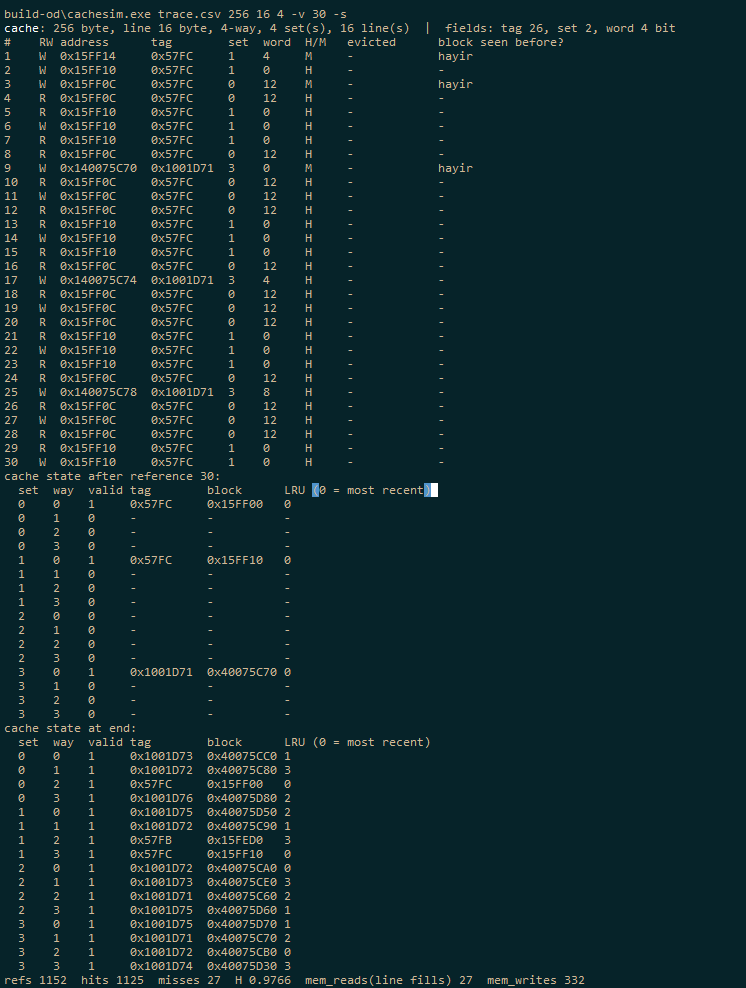
\includegraphics[width=0.8\linewidth]{ss_cache.png}\\[2pt]
{\small Simülatör çıktısı (\tl{ss\_cache.png}): ilk 30 referans, 30.~referanstan sonraki ve
programın sonundaki cache durumu, tüm izin toplamları.}
\end{center}

\textbf{4e. Tasarım uzayı} (cache boyu sabit $=$ 256 byte):

\begin{longtable}{|p{8.6cm}|p{2.0cm}|p{2.0cm}|p{2.0cm}|}
\hline
\hd{Mapping (line boyu sabit $=$ 16 B)} & \hd{Hit} & \hd{Miss} & \hd{H}\\
\hline
Direct & 1098 & 54 & 0,9531\\ \hline
2-way set-associative & 1124 & 28 & 0,9757\\ \hline
4-way set-associative & 1125 & 27 & \textbf{0,9766}\\ \hline
Fully associative (LRU) & 1124 & 28 & 0,9757\\ \hline
\end{longtable}

\begin{longtable}{|p{8.6cm}|p{2.0cm}|p{2.0cm}|p{2.0cm}|}
\hline
\hd{Line boyu (mapping sabit $=$ 4-way)} & \hd{Hit} & \hd{Miss} & \hd{H}\\
\hline
8 B & 1101 & 51 & 0,9557\\ \hline
16 B & 1125 & 27 & 0,9766\\ \hline
32 B & 1136 & 16 & \textbf{0,9861}\\ \hline
64 B & 1135 & 17 & 0,9852\\ \hline
\end{longtable}

\begin{center}
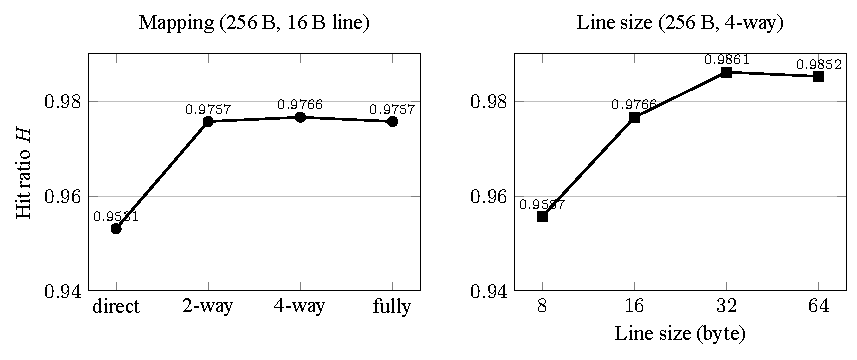
\includegraphics[width=\linewidth]{figures/cache_sweep.pdf}
\end{center}

\textbf{Grafik dosyası ve eğilimlerin locality ile açıklanması} (grafik: \tl{figures/cache\_sweep.pdf}):
\emph{Mapping.} Direct-mapped en kötüsüdür (54 miss): 16 line'lık direct-mapped cache'te
aralarında tam 256 byte'ın katı olan iki blok aynı line'a düşer. \tl{rle\_encode} ve
\tl{rle\_decode}'un stack frame'i (\tl{0x15FEC0}, \tl{0x15FED0}) \tl{v}'nin sonu ve \tl{enc}'in
başıyla (\tl{0x40075CC0}, \tl{0x40075CD0}) aynı line'lara düşer; döngüler her iterasyonda hem
yerel değişkene hem diziye eriştiği için iki blok birbirini sürekli çıkarır (thrashing). Doğrulama
döngüsünde de \tl{v[i]} ile 256 byte ötedeki \tl{dec[i+16]} (\tl{0x40075C70} ve \tl{0x40075D70})
çatışır. 2-way bu çatışmayı büyük ölçüde çözer: aynı set'teki iki blok birlikte durabilir. Fully associative, 4-way'den biraz
\emph{kötüdür}: program 20 farklı bloğa dokunur ama cache 16 line tutar; döngüsel yeniden
erişimde LRU tam da birazdan gerekecek line'ı çıkarır. Yani kalan miss'ler conflict değil
capacity miss'tir. \emph{Line boyu.} 8'den 32 byte'a büyüdükçe H artar: diziler sıralı
taranır, bir miss komşu elemanları da getirir (spatial locality), compulsory miss sayısı düşer.
64 byte'ta H biraz düşer: cache boyu sabit olduğundan yalnızca 4 line kalır (4-way $=$ tek
set); stack, \tl{v}, \tl{dec} ve globaller aynı dört line için yarışır ve temporal locality
kaybedilir. Gerçek L1 cache'lerin 64 byte line kullanması, onların 48 KB gibi çok daha büyük
olmasıyla tutarlıdır.

\textbf{4f. Ortalama erişim süresi:} $T_s = H \times T_1 + (1 - H) \times (T_1 + T_2)$,
$T_1 = 1$, $T_2 = 25$ cycle (varsayım).

\begin{longtable}{|p{4.0cm}|p{2.2cm}|p{3.6cm}|p{5.7cm}|}
\hline
\hd{Durum} & \hd{H} & \hd{$T_s$ (cycle)} & \hd{Speedup (cache'siz duruma göre)}\\
\hline
Cache yok & 0 & $T_2 = $ 25 & 1\\ \hline
Kişiye özel cache & 0,9766 & $0{,}9766 \times 1 + 0{,}0234 \times 26 = $ \textbf{1,586} & $25 / 1{,}586 = $ \textbf{15,76}\\ \hline
\end{longtable}

\textbf{4g. Kod değişikliği:} \tl{main\_v2.c}, \tl{main.c}'den tek bir değişiklikle ayrılır:
\tl{dec}'in eleman tipi 8 bit olur (bunun için diğer tiplerle aynı biçimde bir \tl{u8} typedef'i
eklenir). Makine kodu ve veri erişimleri, \tl{typedef} satırının kaydırdığı C satır numaraları
dışında aynıdır.

\begin{longtable}{|p{6.0cm}|p{4.6cm}|p{4.9cm}|}
\hline
 & \hd{Önce} & \hd{Sonra}\\
\hline
Değiştirilen C satır(lar)ı & s.~17: \tl{s32 dec[N];} & s.~19: \tl{u8 dec[N];} \newline (s.~13: \tl{typedef unsigned char u8;})\\ \hline
Y7 çıktısı (aynı olmalı) & 11, 45, 1 & 11, 45, 1 \checkmark\\ \hline
H & 0,9766 (27 miss) & \textbf{0,9835} (19 miss)\\ \hline
$T_s$ (cycle) & 1,586 & \textbf{1,412}\\ \hline
\end{longtable}

\textbf{Değişikliğin gerekçesi.} Miss analizi, 27 miss'in 7'sinin conflict/capacity olduğunu
gösterdi: program 20 farklı bloğa dokunuyor, cache 16 line tutuyor ve doğrulama döngüsü
\tl{v}'yi yeniden okuduğunda \tl{dec} satırları onu çıkarmış oluyor. \tl{dec} yalnızca 0 ve 1
tutar; byte olarak saklanınca 96 byte'tan 24 byte'a, 6 line'dan 2 line'a iner. Bu hem 4
compulsory miss'i (\tl{dec}'in kalkan 4 line'ı) hem de 4 conflict miss'i siler: toplam ayak izi
16 line'a düşer ve doğrulama döngüsü \tl{v}'yi cache'te bulur. Önce iki başka değişiklik de
denendi ve her biri yalnızca 1 miss kazandırdı: doğrulama döngüsünü tersten yürütmek (LRU'nun
tuttuğu dizi sonlarından başlamak) ve \tl{dec}'i 1--4 line kaydırmak (array padding). İkisinin de
sınırlı kalması, sorunun yanlış set eşlemesi değil kapasite olduğunu gösterdi; bu yüzden ayak
izini küçülten değişiklik seçildi. Bir yan etki: byte karşılaştırması \tl{movzx} gerektirdiği için
\tl{main\_v2} 24 instruction daha fazla yürütür (2112), ama veri referansı sayısı aynıdır (1152).

\textbf{Adım 5 --- Performans ve architecture/organization (final paketiyle: 16 Kasım, Pazartesi)}

\textbf{5a-1. Dinamik instruction dağılımı ve CPI} (CPI\_i değerleri yönergedeki model
varsayımıdır). Sınıflama kuralı: \tl{j*}, \tl{call}, \tl{ret} $\to$ branch; \tl{imul},
\tl{idiv} $\to$ çarpma (modelde bölme sınıfı yoktur, çarpmaya sayılmıştır); belleğe yazan
$\to$ store; bellekten okuyan $\to$ load; geri kalan $\to$ ALU. Kaynak:
\tl{listings/exec\_O0.csv}, \tl{exec\_O1.csv}; hesap \tl{tools/perf.py}.

\begin{longtable}{|p{5.0cm}|p{3.4cm}|p{3.4cm}|p{3.4cm}|}
\hline
\hd{Sınıf} & \hd{CPI\_i (varsayım)} & \hd{I\_i (-O0)} & \hd{I\_i (-O1)}\\
\hline
ALU & 1 & 601 & 601\\ \hline
Çarpma & 3 & 26 & 26\\ \hline
Load & 1 & 792 & 99\\ \hline
Store & 1 & 330 & 68\\ \hline
Branch / jump & 2 & 339 & 194\\ \hline
\textbf{Ic (toplam)} & & \textbf{2088} & \textbf{988}\\ \hline
\textbf{Ortalama CPI} & & \textbf{1,1873} & \textbf{1,2490}\\ \hline
\end{longtable}

\textbf{5a-2. Süre ve MIPS rate} ($f = $ \textbf{1,5} GHz, $\tau = $ \textbf{0,667} ns; varsayım):

\begin{longtable}{|p{4.6cm}|p{4.2cm}|p{3.2cm}|p{3.2cm}|}
\hline
\hd{Ölçü} & \hd{Formül} & \hd{-O0} & \hd{-O1}\\
\hline
T (bellek etkisi yok) & Ic $\times$ CPI $\times$ $\tau$ & 1652,7 ns & 822,7 ns\\ \hline
MIPS rate & $f / (\text{CPI} \times 10^6)$ & 1263,4 & 1201,0\\ \hline
m (instruction başına data referansı) & data ref.\ / Ic & $1152/2088 = 0{,}5517$ & $173/988 = 0{,}1751$\\ \hline
T, cache yok ($k = T_2$) & Ic $\times$ [p $+$ (m $\times$ k)] $\times$ $\tau$ & 20\,852,7 ns & 3\,706,0 ns\\ \hline
T, cache var ($k = T_s$) & Ic $\times$ [p $+$ (m $\times$ k)] $\times$ $\tau$ & 2\,870,7 ns ($T_s = 1{,}586$) & 1\,321,3 ns ($T_s = 4{,}324$)\\ \hline
\end{longtable}

$p$ $=$ ortalama CPI; instruction fetch'lerin 1 cycle'da karşılandığı varsayılmıştır (varsayım).
-O1'in $T_s$'i aynı cache konfigürasyonunda \tl{trace\_O1.csv} ile simüle edilmiştir
(H $=$ 0,8671).

\begin{longtable}{|p{11.0cm}|p{4.5cm}|}
\hline
\hd{Karşılaştırma} & \hd{Değer}\\
\hline
Speedup -O0 $\to$ -O1 (Eq.~2.1, cache var) & $2870{,}7 / 1321{,}3 = $ \textbf{2,17}\\ \hline
Speedup cache yok $\to$ cache var (-O0) & $20852{,}7 / 2870{,}7 = $ \textbf{7,26}\\ \hline
\end{longtable}

\textbf{MIPS rate'in iki derlemeyi karşılaştırmada neden yanıltıcı olabileceği}, kendi
sayılarımla: MIPS'e göre -O0 (1263) -O1'den (1201) \%5 daha ``hızlı'' görünür, oysa -O0 aynı işi
2,11 kat daha fazla instruction'la yapar (2088'e karşı 988) ve gerçekte 2,17 kat yavaştır
(2870,7 ns'ye karşı 1321,3 ns). -O0'ın fazladan instruction'ları çoğunlukla CPI'si 1 olan spill
load/store'larıdır; bunlar ortalama CPI'yi düşürüp MIPS'i yükseltir ama işe katkı yapmaz. MIPS
instruction sayar, iş saymaz; farklı instruction dizileri üreten iki derlemeyi yalnızca toplam
süre (T) adil karşılaştırır. Ayrıca -O0'ın yüksek H'si (0,9766 / 0,8671) da büyük ölçüde stack
trafiğinin sürekli hit olmasından gelir.

\textbf{5a-3. Amdahl yasası} ($N_c = $ \textbf{6}; varsayım):

\begin{longtable}{|p{5.0cm}|p{10.5cm}|}
\hline
\hd{Alan} & \hd{Değer}\\
\hline
\endhead
Paralelleştirilebilen kısım (C satırları) & s.~64--66: doğrulama döngüsü (\tl{for} $\ldots$ \tl{if (dec[i] != v[i]) decode\_ok = 0;})\\ \hline
Bağımsızlık gerekçesi (veri bağımlılığı) & $i$'nci iterasyon yalnızca \tl{dec[i]} ve \tl{v[i]}'yi okur; hiçbir iterasyon başka bir iterasyonun yazdığı değeri okumaz. Tek yazma \tl{decode\_ok = 0}'dır ve hep aynı sabiti yazdığı için sıra önemsizdir (bir AND indirgemesi olarak da yazılabilir). Diğer döngüler seridir: LCG'de $x_{i+1}$, $x_i$'ye bağlıdır; \tl{rle\_encode}'da \tl{i += run} sonraki iterasyonun başlangıcını belirler; \tl{rle\_decode}'da \tl{o} önceki bütün koşuların toplamıdır.\\ \hline
f (yürütme süresindeki pay) & 0,1639 (s.~64--68 instruction'larının cache'li T içindeki payı: $\sum (\text{CPI}_i + m_i \times T_s)$ / toplam; -O0)\\ \hline
Speedup $= 1 / [(1 - f) + f / N_c]$ & $1 / (0{,}8361 + 0{,}1639/6) = $ \textbf{1,158}\\ \hline
$N_c \to \infty$ limiti & $1 / (1 - f) = $ \textbf{1,196}\\ \hline
\end{longtable}

\textbf{5b. Architecture ve organization} (en az 10 özellik). Stallings'in tanımı (Ch.~1.1):
architecture, programcıya görünen ve programın mantıksal yürütülmesini doğrudan etkileyen
özelliklerdir; organization, bu özellikleri gerçekleştiren ve programcıya şeffaf olan
donanım ayrıntılarıdır.

{\small
\begin{longtable}{|p{0.5cm}|p{3.6cm}|p{2.0cm}|p{3.6cm}|p{5.5cm}|}
\hline
\hd{\#} & \hd{Özellik} & \hd{Architecture / Organization} & \hd{Gerekçe (Stallings tanımı)} & \hd{Değişseydi Y7 değişir miydi? Kanıt}\\
\hline
\endhead
1 & Instruction set ve encoding (x86-64, 1--15 byte) & Architecture & Derleyici ve programcı bunu görür, programın anlamını belirler & Yeniden derlenmeden çalışmaz; derlenince aynı: -O0 ve -O1 farklı instruction dizileri, Y7 aynı (2b)\\ \hline
2 & Genel amaçlı register sayısı (16) & Architecture & Programcıya görünür & Hayır (derlenince): -O0 4, -O1 7 register kullanır, Y7 aynı\\ \hline
3 & Adresleme modları (base $+$ index$\times$scale $+$ disp, RIP-relative) & Architecture & Instruction anlamının parçası & Hayır: -O1 farklı modlar (\tl{[rax+rcx]}) kullanır, Y7 aynı\\ \hline
4 & Tamsayı genişliği (\tl{int} 32 bit, mod $2^{32}$ aritmetik) & Architecture & Veri tiplerinin bit sayısı (Stallings'in örneği) & \textbf{Evet}: LCG mod $2^{32}$ taşmaya dayanır. 16 bit aritmetikte \tl{x >> 16} hep 0 olur, \tl{v} tamamen 0 çıkar ve Y7 $=$ (1, 4, 1) olur\\ \hline
5 & Interrupt mekanizması (IDT, vektör, stack frame) & Architecture & Sistem programcısına görünür & Hayır: interrupt programa şeffaftır, bağlam aynen geri yüklenir (3c)\\ \hline
6 & Byte sırası (little-endian) & Architecture & Bellekteki veri biçimi programcıya görünür & Hayır: program hiçbir değişkeni byte byte yorumlamaz; yalnızca makine kodu düzeni değişir (2c)\\ \hline
7 & Cache boyu (256 B) & Organization & Programcıya şeffaf donanım & Hayır: aşağıdaki tabloda 7 konfigürasyonda iz aynı, yalnızca H ve süre değişir\\ \hline
8 & Mapping (4-way set-assoc.) & Organization & Programcıya şeffaf & Hayır (4e)\\ \hline
9 & Line boyu (16 B) & Organization & Programcıya şeffaf & Hayır (4e)\\ \hline
10 & Write policy (write-through) & Organization & Programcıya şeffaf & Hayır: yalnızca ana belleğe yazma sayısı değişir (332)\\ \hline
11 & Data bus genişliği (64 bit) & Organization & Aktarım genişliği bir gerçekleştirme ayrıntısıdır & Hayır: yalnızca bus cycle sayısı değişir (26 $\to$ 58, 3d)\\ \hline
12 & Saat frekansı (1,5 GHz) & Organization & Programcıya şeffaf & Hayır: yalnızca $T = \text{Ic} \times \text{CPI} / f$ değişir\\ \hline
13 & Çarpma donanımı (\tl{imul}'un gerçekleştirilişi, CPI 3) & Organization & Stallings: çarpma instruction'ının varlığı architecture, nasıl yapıldığı organization & Hayır: yalnızca cycle sayısı değişir\\ \hline
14 & Fiziksel adres genişliği (bu CPU'da 39 bit) & Organization & Aynı ISA (64 bit adres) farklı gerçekleştirmeler & Hayır: programın adresleri 33 bite sığar\\ \hline
\end{longtable}
}

\textbf{Son sütunun testi:} Aşama 4'teki bütün cache konfigürasyonları aynı \tl{trace.csv}'yi
işler; cache değerleri değil yalnızca erişim süresini değiştirir, Y7 her birinde (11, 45, 1)
kalır. Süre ise değişir ($T$, -O0, cache var):

\begin{longtable}{|p{5.0cm}|p{2.0cm}|p{2.6cm}|p{2.6cm}|p{3.3cm}|}
\hline
\hd{Konfigürasyon (256 B)} & \hd{H} & \hd{$T_s$ (cycle)} & \hd{$T$ (ns)} & \hd{Y7}\\
\hline
direct, 16 B & 0,9531 & 2,172 & 3320,7 & 11, 45, 1\\ \hline
2-way, 16 B & 0,9757 & 1,608 & 2887,4 & 11, 45, 1\\ \hline
4-way, 16 B (kişiye özel) & 0,9766 & 1,586 & 2870,7 & 11, 45, 1\\ \hline
fully, 16 B & 0,9757 & 1,608 & 2887,4 & 11, 45, 1\\ \hline
4-way, 8 B & 0,9557 & 2,107 & 3270,7 & 11, 45, 1\\ \hline
4-way, 32 B & 0,9861 & 1,347 & 2687,4 & 11, 45, 1\\ \hline
4-way, 64 B & 0,9852 & 1,369 & 2704,1 & 11, 45, 1\\ \hline
\end{longtable}

\textbf{Ch.~1.2'deki dört temel fonksiyon:}

\begin{longtable}{|p{2.8cm}|p{5.2cm}|p{7.5cm}|}
\hline
\hd{Fonksiyon} & \hd{Kernel'den örnek instruction (adres, assembly)} & \hd{Açıklama}\\
\hline
Data processing & \tl{0x140001209} \tl{idiv ecx} & ALU veriyi işler: $1100 \div 24 = 45$\\ \hline
Data storage & \tl{0x14000120B} \tl{mov [rip+0x74A53], eax} & Sonuç (\tl{ratio\_x100}) belleğe yazılır ve program bittikten sonra orada kalır (Y7)\\ \hline
Data movement & \tl{0x140001168} \tl{mov eax, [rsp+0x10]} & Veri bellekten register'a taşınır. Program dış dünyayla I/O yapmaz; Stallings'in anlamındaki dışarıya taşıma, sonuçların bellekten debugger ile okunmasıyla olur\\ \hline
Control & \tl{0x140001170} \tl{ret} ve \tl{0x140001231} \tl{jge} & Instruction akışını yönetir: dönüş adresine sıçrama, koşullu dallanma\\ \hline
\end{longtable}

\textbf{Final teslim (16 Kasım Pazartesi; sözlü savunma 20 Kasım Cuma)}

\textbf{Teslim kontrol listesi:}

\begin{itemize}[leftmargin=2em,itemsep=1pt,topsep=2pt]
\item $\boxtimes$ Bu tutanak, tüm adımları dolu olarak (PDF: \tl{CMPE3209\_Tutanak.pdf}, düzenlenebilir sürüm: \tl{CMPE3209\_Tutanak.tex})
\item $\boxtimes$ C kaynak kodu (\tl{main.c}) ve sonraki 4g sürümü (\tl{main\_v2.c})
\item $\boxtimes$ \tl{asm\_O0.s}, \tl{asm\_O1.s} ve objdump -d çıktısı (\tl{listings/})
\item $\boxtimes$ \tl{trace.csv} ve cache simülasyon çıktıları (\tl{listings/cachesim\_report.txt}; simülatör kaynağı \tl{tools/cachesim.c})
\item $\boxtimes$ Ekran görüntüleri: machine code doğrulaması (\tl{ss\_m2\_disasm.png}), program çıktıları (\tl{ss\_globals.png}), cache durumu (\tl{ss\_cache.png})
\item $\boxtimes$ 4e grafiği (\tl{figures/cache\_sweep.pdf})
\item $\square$ Git deposunda M1, M2 ve final etiketleri
\end{itemize}

\textbf{Kilometre taşı kaydı} (öğretim üyesi doldurur):

\begin{longtable}{|p{4.4cm}|p{4.2cm}|p{2.4cm}|p{2.2cm}|p{1.6cm}|}
\hline
\hd{Kilometre taşı} & \hd{Son tarih} & \hd{Teslim tarihi} & \hd{Git etiketi} & \hd{Paraf}\\
\hline
M1 Öneri (Adım 0--1) & 2 Kasım (Pzt) & & & \\ \hline
M2 Assembly ve machine code (Adım 2) & 9 Kasım (Pzt) & & & \\ \hline
M3 CPU, interrupt, bus (Adım 3) & 16 Kasım (Pzt, final paketiyle) & & & \\ \hline
M4 Cache ve performans (Adım 4--5) & 16 Kasım (Pzt, final paketiyle) & & & \\ \hline
Final ve sözlü savunma & Teslim 16 Kasım (Pzt); savunma 20 Kasım (Cuma) & & & \\ \hline
\end{longtable}

\textbf{YZ kullanım beyanı.} Kullanılmadıysa ilk satıra ``Kullanılmadı'' yazın. Beyan edilmemiş
kullanım akademik dürüstlük ihlalidir.

\begin{longtable}{|p{2.8cm}|p{1.4cm}|p{3.6cm}|p{3.4cm}|p{3.8cm}|}
\hline
\hd{Araç ve sürümü} & \hd{Adım} & \hd{Ne için kullanıldı} & \hd{Örnek prompt} & \hd{Çıktıyı nasıl doğruladım}\\
\hline
Claude Code (Anthropic, Claude Opus) & 0--5 & Rapor yazımında yardımcı: tutanağın Türkçe metni, tablo ve LaTeX dizgisi; Intel SDM Vol.~3A'daki interrupt mekanizması için bölüm ve sayfa referanslarının bulunması (3c) & ``Tutanağı resmi forma benzer biçimde doldur''; ``Intel SDM'de 64-bit mode interrupt stack frame bölümünü ve sayfasını bul'' & Metindeki her sayıyı kendi derleme, debugger ve simülasyon çıktılarımla karşılaştırdım; SDM referanslarını 253668-080US PDF'inin içindekiler tablosundan kontrol ettim\\ \hline
Claude Code (Anthropic, Claude Opus) & 2, 4, 5 & Yardımcı araçların yazılması: \tl{tools/mktrace.py} (debugger kaydından \tl{trace.csv}), \tl{tools/c2asm.py} (C satırı $\to$ adres eşlemesi), \tl{tools/perf.py} (5a hesapları), \tl{cmake/listings.cmake} (listeleme) & ``Debugger'ın tek adım kaydından her load ve store için etkin adresi hesaplayıp trace.csv yazan bir Python scripti yaz'' & İz M1'deki ölçümle birebir tutar (1152 referans, 961 stack); iki ayrı çalıştırma aynı izi verir; simülatör ilk 30 referansta elle simülasyonla örtüşür; makine kodu objdump ve Visual Studio ile aynıdır. Cache simulatorü şahsım tarafından yazılmıştır.\\ \hline
\end{longtable}

\textbf{Öğrenci beyanı.} Bu tutanaktaki C kodunu, elle machine code kodlamasını, instruction cycle
izleme tablosunu ve elle cache simülasyonunu kendim yaptım. Başka bir öğrencinin çalışmasını
kopyalamadım ve kendi çalışmamı paylaşmadım. YZ kullanımımı eksiksiz beyan ettim. Sözlü savunmada
bu çalışmayı açıklayamamamın puanımı etkileyeceğini biliyorum.

\begin{longtable}{|p{4.4cm}|p{4.4cm}|p{3.0cm}|p{3.0cm}|}
\hline
\hd{Ad Soyad} & \hd{Öğrenci numarası} & \hd{Tarih} & \hd{İmza}\\
\hline
Mehmet Batuhan Özer & 5001230025 & & \\ \hline
\end{longtable}

\textbf{Değerlendirme} (öğretim üyesi doldurur)

\begin{longtable}{|p{8.4cm}|p{2.0cm}|p{2.0cm}|p{2.4cm}|}
\hline
\hd{Bileşen} & \hd{Azami} & \hd{Puan} & \hd{Not}\\
\hline
A1 Öneri ve parametre hesabı (Adım 0--1) & 5 & & \\ \hline
A2 Assembly ve machine code (Adım 2) & 15 & & \\ \hline
A3 CPU, interrupt, bus (Adım 3) & 25 & & \\ \hline
A4 Cache (Adım 4) & 25 & & \\ \hline
A5 Performans ve architecture/organization (Adım 5) & 10 & & \\ \hline
Tutanak ve rapor kalitesi & 5 & & \\ \hline
Sözlü savunma & 15 & & \\ \hline
Geç teslim kesintisi & --- & & \\ \hline
\textbf{Toplam} & \textbf{100} & & \\ \hline
\end{longtable}

\textbf{Sözlü savunma kaydı:}

\begin{longtable}{|p{6.0cm}|p{2.0cm}|p{5.0cm}|p{1.8cm}|}
\hline
\hd{Madde} & \hd{Sorulan} & \hd{Sonuç (başarılı / kısmen / başarısız)} & \hd{Puan}\\
\hline
1. Canlı encode (-O1 listesinden) & & & \\ \hline
2. Adres alanları ve hit/miss & & & \\ \hline
3. Interrupt k$+$1'de gelseydi & & & \\ \hline
4. Tasarım kararı savunması & & & \\ \hline
\end{longtable}

$\square$ 1. ve 2. maddelerin ikisi de başarısız: A2--A4 puanları 0.5 ile çarpıldı.

\begin{longtable}{|p{7.6cm}|p{3.6cm}|p{3.6cm}|}
\hline
\hd{Öğretim üyesi} & \hd{Tarih} & \hd{İmza}\\
\hline
 & & \\ \hline
\end{longtable}

\end{document}
